%% 
%% Copyright 2007-2025 Elsevier Ltd
%% 
%% This file is part of the 'Elsarticle Bundle'.
%% ---------------------------------------------
%% 
%% It may be distributed under the conditions of the LaTeX Project Public
%% License, either version 1.3 of this license or (at your option) any
%% later version.  The latest version of this license is in
%%    http://www.latex-project.org/lppl.txt
%% and version 1.3 or later is part of all distributions of LaTeX
%% version 1999/12/01 or later.
%% 
%% The list of all files belonging to the 'Elsarticle Bundle' is
%% given in the file `manifest.txt'.
%% 
%% Template article for Elsevier's document class `elsarticle'
%% with numbered style bibliographic references
%% SP 2008/03/01
%% $Id: elsarticle-template-num.tex 272 2025-01-09 17:36:26Z rishi $
%%
%\documentclass[preprint,12pt]{elsarticle}

%% Use the option review to obtain double line spacing
%% \documentclass[authoryear,preprint,review,12pt]{elsarticle}

%% Use the options 1p,twocolumn; 3p; 3p,twocolumn; 5p; or 5p,twocolumn
%% for a journal layout:
\documentclass[final,1p,times]{elsarticle}
%% \documentclass[final,1p,times,twocolumn]{elsarticle}
%% \documentclass[final,3p,times]{elsarticle}
%% \documentclass[final,3p,times,twocolumn]{elsarticle}
%% \documentclass[final,5p,times]{elsarticle}
%% \documentclass[final,5p,times,twocolumn]{elsarticle}

%% For including figures, graphicx.sty has been loaded in
%% elsarticle.cls. If you prefer to use the old commands
%% please give \usepackage{epsfig}

%% The amssymb package provides various useful mathematical symbols
\usepackage{amssymb}
%% The amsmath package provides various useful equation environments.
\usepackage{amsmath}
%% The amsthm package provides extended theorem environments
%% \usepackage{amsthm}
\usepackage{hyperref}

% User-added packages
\usepackage{listings}
\usepackage{array}
\usepackage{xcolor}
\usepackage{soul}
\usepackage{booktabs}
%\usepackage{manyfoot}%
%\usepackage{footnote}
%\makesavenoteenv{tabular}  % if using footnotes inside tabular
\usepackage{tabularx}
\usepackage{geometry}
\usepackage{threeparttable}
\usepackage[nolist]{acronym}
\usepackage[figuresright]{rotating} % include this in your preamble
\usepackage{adjustbox}
\usepackage{tablefootnote}

% Define a muted color palette
\definecolor{codebg}{RGB}{253, 253, 253}
\definecolor{keywordcolor}{RGB}{30,60,114}
\definecolor{stringcolor}{RGB}{50,100,50}
\definecolor{commentcolor}{RGB}{150,150,150}
\definecolor{identifiercolor}{RGB}{40,40,40}
\definecolor{codegreen}{rgb}{0,0.6,0}
\definecolor{codegray}{rgb}{0.5,0.5,0.5}
\definecolor{codepurple}{rgb}{0.58,0,0.82}
\definecolor{backcolour}{rgb}{0.95,0.95,0.92}
\definecolor{darkred}{rgb}{0.6,0.0,0.0}
\definecolor{darkgreen}{rgb}{0,0.50,0}
\definecolor{lightblue}{rgb}{0.0,0.42,0.91}
\definecolor{orange}{rgb}{0.99,0.48,0.13}
\definecolor{grass}{rgb}{0.18,0.80,0.18}
\definecolor{pink}{rgb}{0.97,0.15,0.45}

% Custom command definitions
%\newcommand*{\figref}[2][]{%
%  \hyperref[{#2}]{%
%    \ref*{#2}%
%    \ifx\\#1\\%
%    \else
%      #1%
%    \fi
%  }%
%}

% General Setting of listings
\lstset{
  aboveskip=1em,
  breaklines=true,
  abovecaptionskip=6pt,
  captionpos=b,
  escapeinside={\%*}{*)},
  frame=single,
  numbers=left,
  numbersep=10pt,
  tabsize=2,
  keepspaces=true,                                    
  showspaces=false,                
  showstringspaces=false,
  showtabs=false,
  numberstyle=\tiny,
  breakatwhitespace=false,         
  breaklines=true,
  basicstyle=\ttfamily, %\footnotesize
}
% 1. General Python Keywords List
\lstdefinelanguage{PythonReemission}[]{Python}{
  morekeywords=[1]{,as,assert,nonlocal,with,yield,self,True,False,None,} % Python builtin
  morekeywords=[2]{,__init__,__add__,__mul__,__div__,__sub__,__call__,__getitem__,__setitem__,__eq__,__ne__,__nonzero__,__rmul__,__radd__,__repr__,__str__,__get__,__truediv__,__pow__,__name__,__future__,__all__,}, % magic methods
  morekeywords=[3]{,object,type,isinstance,copy,deepcopy,zip,enumerate,reversed,list,set,len,dict,tuple,range,xrange,append,execfile,real,imag,reduce,str,repr,}, % common functions
  morekeywords=[4]{,Exception,NameError,IndexError,SyntaxError,TypeError,ValueError,OverflowError,ZeroDivisionError,}, % errors
  morekeywords=[5]{,ode,fsolve,sqrt,exp,sin,cos,arctan,arctan2,arccos,pi, array,norm,solve,dot,arange,isscalar,max,sum,flatten,shape,reshape,find,any,all,abs,plot,linspace,legend,quad,polyval,polyfit,hstack,concatenate,vstack,column_stack,empty,zeros,ones,rand,vander,grid,pcolor,eig,eigs,eigvals,svd,qr,tan,det,logspace,roll,min,mean,cumsum,cumprod,diff,vectorize,lstsq,cla,eye,xlabel,ylabel,squeeze,},
  emph={,ReemissionEngine, MonthlyTemperature, CarbonDioxideEmission, NitrousOxideEmission, MethaneEmission, Landuse, Climate, SoilType, Biome, TreatmentFactor, LanduseIntensity, Catchment, Reservoir, BiogenicFactors}, % numpy / math
}

% 3. Extended theme
\lstdefinestyle{colorEX}{
  basicstyle=\ttfamily\footnotesize,
  backgroundcolor=\color{codebg},
  commentstyle=\color{darkgreen}\slshape,
  keywordstyle=\color{blue}\bfseries\itshape,
  keywordstyle=[2]\color{blue}\bfseries,
  keywordstyle=[3]\color{grass},
  keywordstyle=[4]\color{red},
  keywordstyle=[5]\color{orange},
  stringstyle=\color{darkred},
  emphstyle=\color{pink}\underbar,
  numberstyle=\tiny\color{codegray},
  numbersep=10pt,
}
\lstdefinestyle{custmpythonstyle}{
    backgroundcolor=\color{codebg},
    commentstyle=\color{commentcolor}\itshape,
    keywordstyle=\color{keywordcolor}\bfseries,
    stringstyle=\color{stringcolor},
    identifierstyle=\color{identifiercolor},
    breaklines=true,
    captionpos=b,
    keepspaces=true,
    numbers=left,
    frame=single,
    numbersep=10pt,
    rulecolor=\color{gray},
    showstringspaces=false
}

\lstdefinelanguage{Dockerfile}{
  morekeywords={FROM, RUN, CMD, LABEL, MAINTAINER, EXPOSE, ENV, ADD, COPY, ENTRYPOINT, VOLUME, USER, WORKDIR, ARG, ONBUILD, STOPSIGNAL, HEALTHCHECK, SHELL},
  sensitive=true,
  morecomment=[l]{\#},
  morestring=[b]"
}

\lstset{style=colorEX}

%% The lineno packages adds line numbers. Start line numbering with
%% \begin{linenumbers}, end it with \end{linenumbers}. Or switch it on
%% for the whole article with \linenumbers.
%% \usepackage{lineno}

\usepackage{caption}
\captionsetup[lstlisting]{font=small}
\captionsetup[table]{font=normalsize}
\captionsetup[figure]{font=normalsize}
\captionsetup[bibliography]{font=normalsize}

\usepackage[linesnumbered,ruled,vlined]{algorithm2e}

\usepackage{refcount}  % for \getrefnumber
\usepackage{xparse}    % for optional arguments
\NewDocumentCommand{\figref}{O{}m}{%
  \hyperref[#2]{\ref*{#2}#1}%
}

%\NewDocumentCommand{\figref}{O{}m}{%
%  \getrefnumber{#2}#1%
%}

% This will be executed when \appendix is called
\AtBeginDocument{%
  \let\oldappendix\appendix
  \renewcommand{\appendix}{%
    \oldappendix
    % Reset counters
    \setcounter{figure}{0}
    \setcounter{table}{0}
    \setcounter{equation}{0}
    \setcounter{lstlisting}{0}
    
    % Redefine the counter representation
    \renewcommand{\thefigure}{A.\arabic{figure}}
    \renewcommand{\thetable}{A.\arabic{table}}
    \renewcommand{\theequation}{A.\arabic{equation}}
    \renewcommand{\thelstlisting}{A.\arabic{lstlisting}}
  }
}

\makeatletter
\newcommand{\vrbbrk}[1]{%
  \begingroup
  \ttfamily
  \begingroup\lccode`~=`/\lowercase{\endgroup\def~}{/\discretionary{}{}{}}%
  \begingroup\lccode`~=`[\lowercase{\endgroup\def~}{[\discretionary{}{}{}}%
  \begingroup\lccode`~=`.\lowercase{\endgroup\def~}{.\discretionary{}{}{}}%
  \catcode`/=\active\catcode`[=\active\catcode`.=\active
  \scantokens{#1\noexpand}%
  \endgroup
}
\makeatother


\journal{Environmental Modelling \& Software}

\begin{document}

\begin{frontmatter}

%% Title, authors and addresses

%% use the tnoteref command within \title for footnotes;
%% use the tnotetext command for theassociated footnote;
%% use the fnref command within \author or \affiliation for footnotes;
%% use the fntext command for theassociated footnote;
%% use the corref command within \author for corresponding author footnotes;
%% use the cortext command for theassociated footnote;
%% use the ead command for the email address,
%% and the form \ead[url] for the home page:
%% \title{Title\tnoteref{label1}}
%% \tnotetext[label1]{}
%% \author{Name\corref{cor1}\fnref{label2}}
%% \ead{email address}
%% \ead[url]{home page}
%% \fntext[label2]{}
%% \cortext[cor1]{}
%% \affiliation{organization={},
%%             addressline={},
%%             city={},
%%             postcode={},
%%             state={},
%%             country={}}
%% \fntext[label3]{}

\title{\emph{Re-Emission}: A free open-source software for estimating, reporting, and visualizing greenhouse gas emissions from reservoirs}

%% use optional labels to link authors explicitly to addresses:
 \author[label1]{Tomasz Janus}
 \affiliation[label1]{organization={Tyndall Centre Manchester, University of Manchester},
             addressline={Floor 5, Engineering A, Booth Street East},
             city={Manchester},
             postcode={M13 9PL},
             %state={},
             country={United Kingdom}}
 \author[label2]{Christopher Barry}
 \affiliation[label2]{organization={UK Centre for Ecology \& Hydrology},
             addressline={Deiniol Road},
             city={Bangor},
             postcode={LL57 2UW},
             %state={},
             country={United Kingdom}}           
 \author[label3,label4]{Xingxing Zhang}
 \affiliation[label3]{organization={State Key Laboratory of Resources and Environmental Information System, Institute of Geographic Sciences and Natural Resources Research},
             addressline={Chinese Academy of Sciences},
             city={Beijing},
             %postcode={M13 9PL},
             %state={},
             country={China}}
 \affiliation[label4]{organization={College of Resources and Environment},
             addressline={University of Chinese Academy of Sciences},
             city={Beijing},
             %postcode={M13 9PL},
             %state={},
             country={China}} 
 \author[label1]{Jaise Kuriakose}           

%% Abstract
\begin{abstract}
Reservoirs are significant contributors to anthropogenic \ac{GHG} emissions, whose broad impacts on the climate warrant appropriate assessment and reporting. 
However, existing tools for estimating reservoir emissions are often limited in scope or require extensive input data and manual processing, restricting their application to small sets of reservoirs.
Here, we present \emph{Re-Emission}, a free and open-source tool that streamlines the modelling of reservoir emissions, offers custom configuration options, and enables estimation at regional to national scales.  
We demonstrate its utility through two case studies involving approximately 250 reservoirs.
\emph{Re-Emission} can be integrated into broader multi-domain frameworks, supporting applications in domains such as water resources and energy planning. 
It interfaces with a catchment analysis tool to automate reservoir emission assessments, eliminating the need for extensive user input -- a key barrier to a wider adoption of spatially-explicit emission models.
\end{abstract}

%%Graphical abstract
\begin{graphicalabstract}
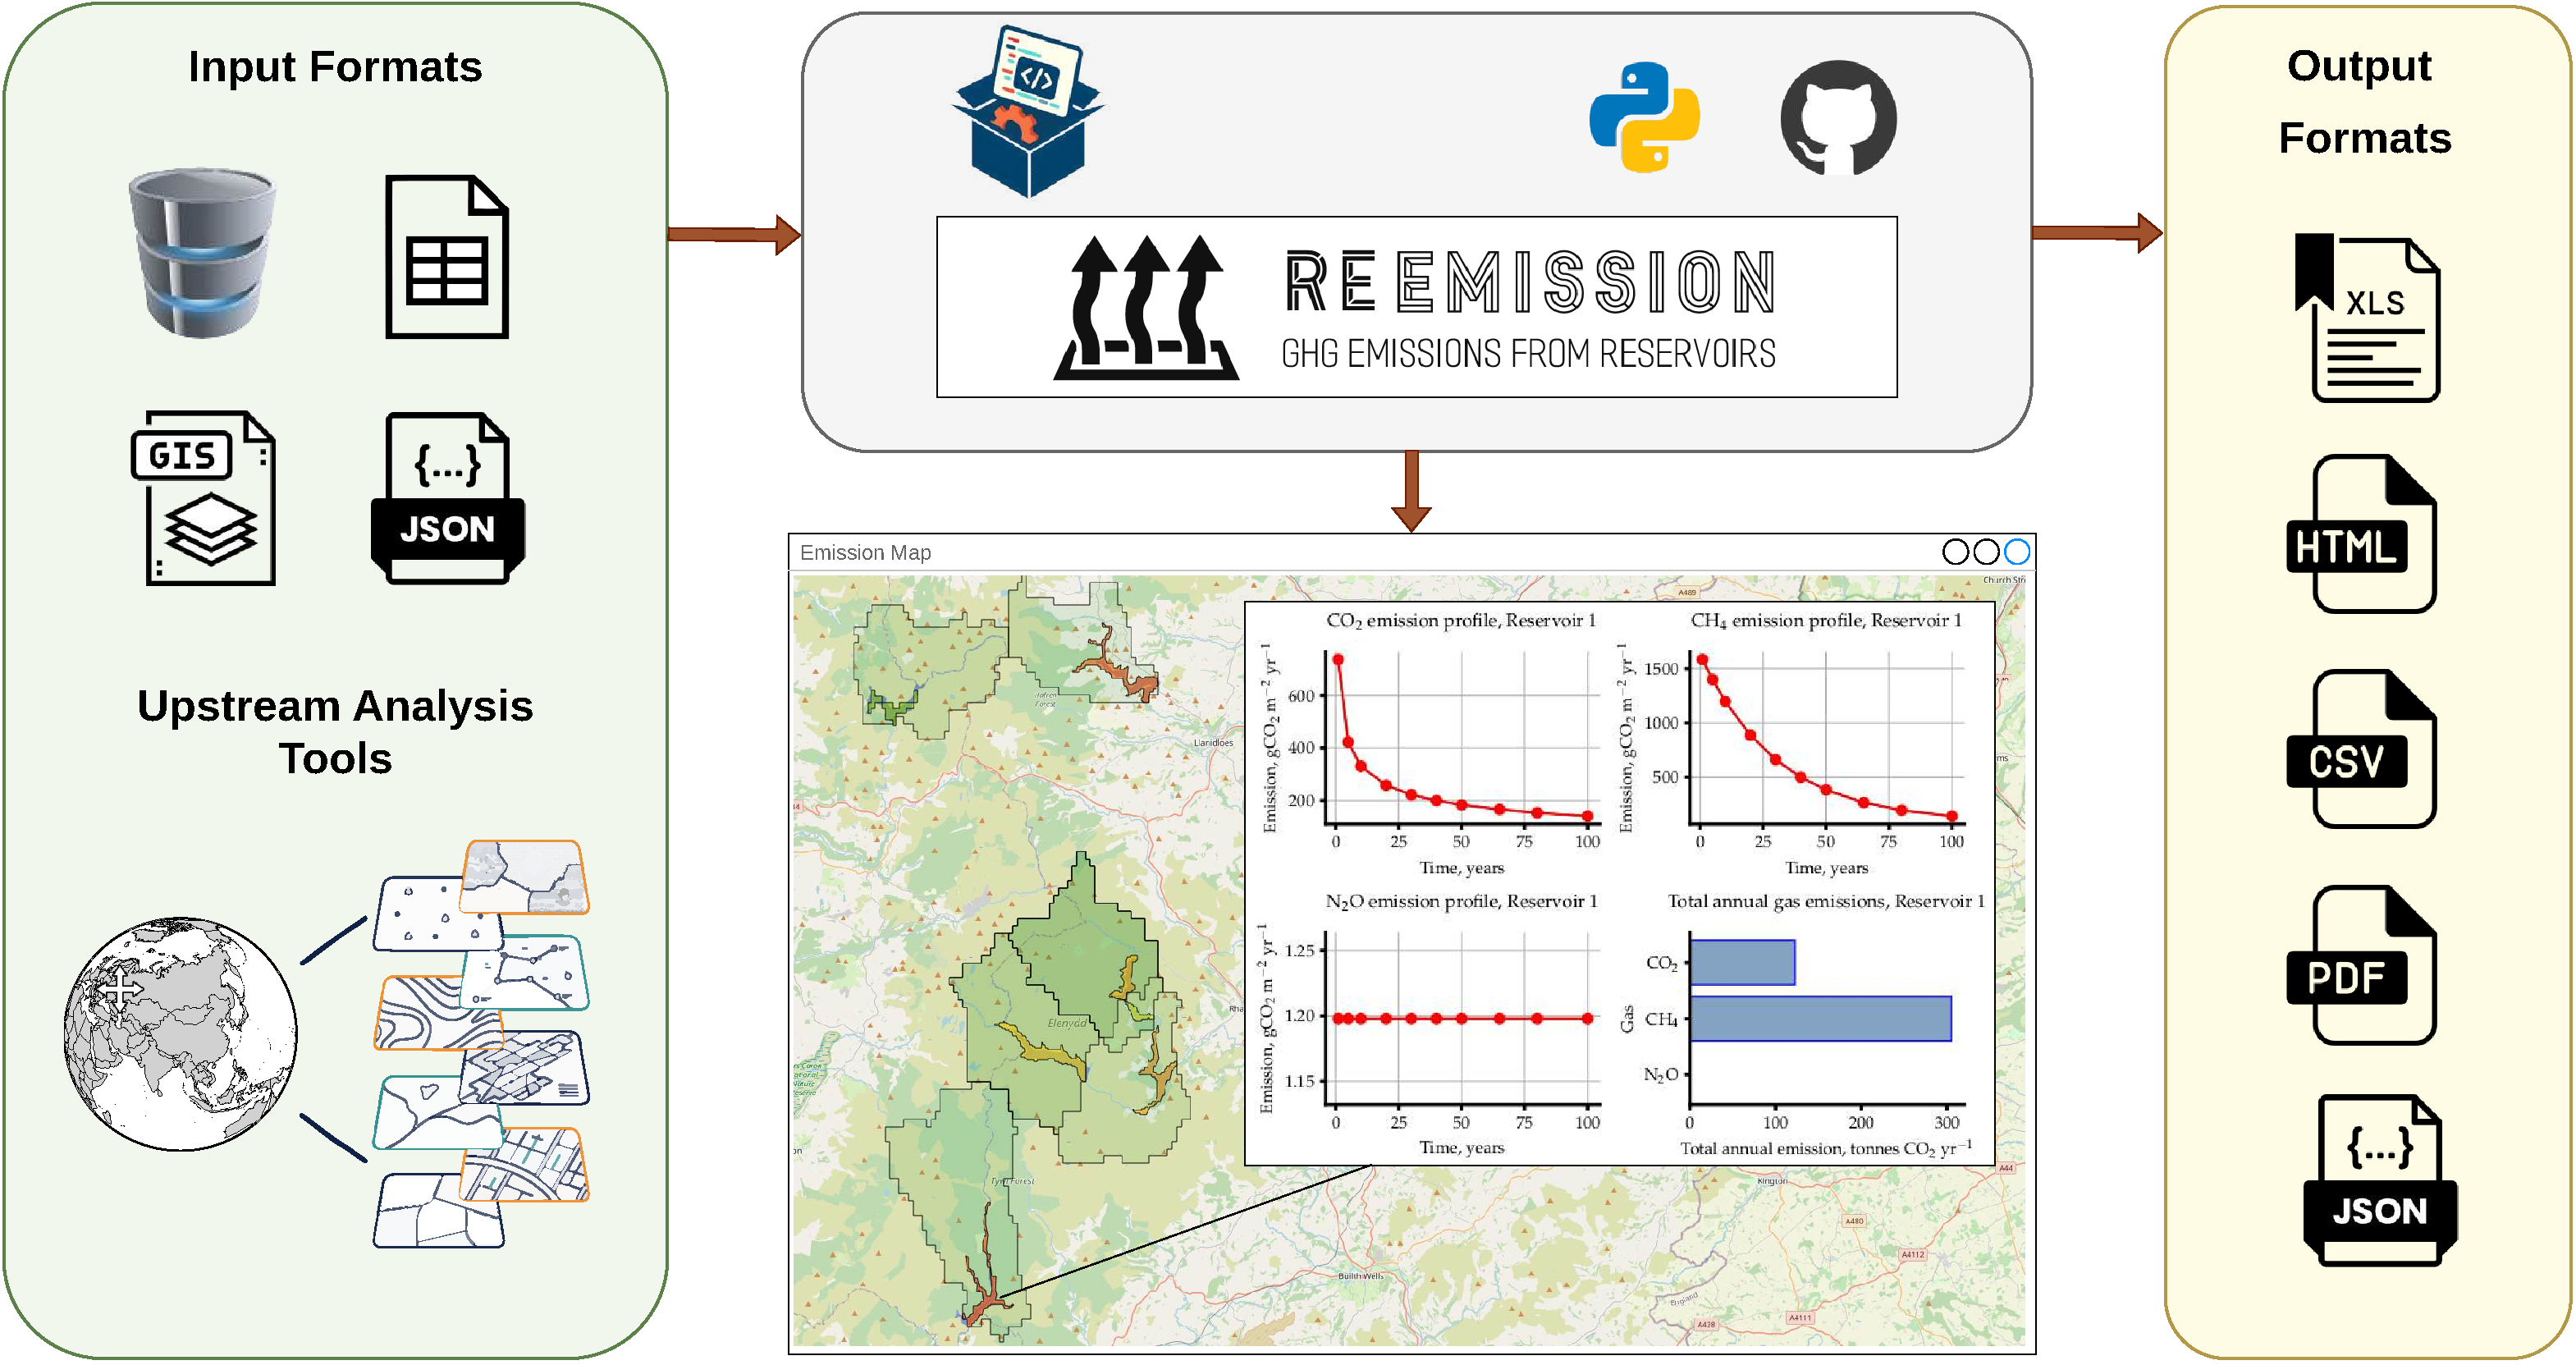
\includegraphics[width=1\textwidth]{figures/graphical_abstract_new.drawio-compressed.pdf}
\end{graphicalabstract}

%%Research highlights
\begin{highlights}
\item Command line tool and a Python library for calculating reservoir emissions.
\item Configurable calculation and visualization options.
\item Integrates with \acs{GIS}-based catchment and reservoir delineation tool.
%\item Automates emission calculations from multiple reservoirs.
\item Supports multiple output and report formats.
\item Applications in the United Kingdom and Myanmar highlight Re-Emission's features.
\end{highlights}

%% Keywords
\begin{keyword}
automated assessments \sep greenhouse gas emissions \sep reservoirs \sep open source
%% keywords here, in the form: keyword \sep keyword
%% PACS codes here, in the form: \PACS code \sep code
%% MSC codes here, in the form: \MSC code \sep code
%% or \MSC[2008] code \sep code (2000 is the default)
\end{keyword}

\end{frontmatter}

\section{Introduction}
\label{sec:introduction}

Reservoirs are increasingly recognized as significant sources of biogenic \ac{GHG} emissions~\citep{Barros2011}, particularly in low-altitude tropical regions where the emission intensities of hydroelectric dams (e.g., kg~CO$_{2e}$\,MWh$^{-1}$) may exceed those of fossil fuel power plants~\citep{Fearnside2002}. 
These emissions arise from the decomposition of organic matter that was either flooded during reservoir construction, transported into the reservoir by riverine runoff, or produced in situ through processes such as algal growth~\citep{Louis2000}.
Recent estimates suggest that reservoirs contribute approximately 5.2\% of global anthropogenic \ac{CH4} emissions and 0.2\% of \ac{CO2} emissions, together accounting for 1-2\% of total anthropogenic \ac{GHG} emissions~\citep{Soued2022}.
Ongoing and planned investments in reservoir infrastructure are likely to impede progress toward achieving the climate targets set by the Paris Agreement.
In the hydroelectric sector alone, more than 3,700 new dams are planned~\citep{Zarfl2015,Bouckaert2021}, potentially adding approximately 400\,MtCO$_{2e}$ annually to global emissions~\citep{janus2025planning} -- an amount equivalent to around 11\% of the European Union’s current emissions.
Projections for planned reservoir investments in sectors such as flood control and water supply are less well known but are likely to be substantial, driven by efforts to enhance the resilience of water resource systems to climatic uncertainty~\cite{ipcc2018, Sarkodie2022}.
Given the potentially high areal \ac{GHG} fluxes from reservoirs, rigorous emission estimation is needed both (i) for planned reservoirs, to enable the design of low-carbon expansion strategies, and (ii) for existing reservoirs, to improve the accuracy of global \ac{GHG} inventories.


%Although several estimates of the total number and total area of reservoirs worldwide have been constructed, contemporary advances in remote sensing and global hydrological mapping have considerably increased our understanding of their true extent and distribution.
%\citet{Downing2006} estimated the number of impoundments globally at 515,149 with a total area of 258,570~km$^2$
%More recent studies provide significantly higher estimates: $\sim$2.8 million reservoirs with a total area of $\sim$530,000~km$^2$~\cite{Mulligan2020} and $\sim$2.5 million with $\sim$642,000~km$^2$ total surface area~\cite{LehnerMessager2023}. 
%All of the above figures are considerably larger than those reported in global dam databases such as \acs{FHReD}~\cite{Zarfl2015FHReD} ($\sim$40,000), \acs{GOOD2}~\cite{Mulligan2021GOOD2} ($\sim$38,667), or \acs{ICOLD}~\cite{ICOLD2020} ($\sim$58,700). 
%These discrepancies stem largely from improved satellite imagery and detection methods that can now identify millions of small and previously undocumented reservoirs.
%Given the likely exclusion of numerous existing reservoirs with unquantified atmospheric impacts, current global emission estimates may require reassessment to account for these new contributions.

Several studies have addressed the methodological challenges of quantifying reservoir emissions and have provided estimates of \ac{GHG} emissions from existing reservoirs at both global~\citep{Barros2011, Soued2022, Deemer2016, Prairie2018, Harrison2021} and regional scales~\citep{Hidrovo2017, Rasanen2018, Almeida2019, Hansen2022}. 
These studies have shown that emissions are shaped by a complex interplay of hydro-morphological, edaphic, climatic, and land-use characteristics of reservoirs and their catchments~\citep{Deemer2016, Prairie2021}.
Nevertheless, current global assessments, including the most recent~\citep{Harrison2021, Soued2022}, rely on empirical flux approximations derived from a limited number of measured sites, rather than on the application of spatially explicit emission models to individual reservoirs.
Such approaches are unable to capture the variability in emission fluxes driven by site-specific environmental conditions and reservoir properties~\citep{janus2025planning}, which in turn may undermine the reliability of global emission inventories and strategic planning efforts. 
Moreover, the underlying measurement data used for upscaling are typically biased toward large, deep hydroelectric reservoirs~\citep{Hansen2022}, underrepresenting small, shallow reservoirs~\citep{Malerba2022} -- which are often rich in organic matter and more conducive to elevated methane production~\citep{WANG2025123441, SHI2025}. 
As a result, the global \acp{EF} derived in recent assessments~\citep{Harrison2021, Soued2022} may underestimate emissions from small, shallow reservoirs such as those used for irrigation, thereby introducing bias into global reservoir emission estimates.

A major barrier to addressing the challenges outlined above is the lack of software capable of estimating reservoir emissions at national, regional, and global scales using the most up-to-date emission models that go beyond Tier~1 \acf{EF} approaches and basic upscaling techniques.
The most comprehensive and widely recognized model for estimating reservoir \ac{GHG} emissions is the G-res model~\citep{Prairie2017b, Prairie2021}, which provides spatially explicit estimates of both gross and net emissions by accounting for anthropogenic and natural sources, as well as a broad range of climatic, hydro-morphological, edaphic, and land-use drivers.
G-res is implemented through a publicly available web-based platform, the G-res Tool~\citep{prairie2017gres}, which offers free assessments for non-commercial users and paid services for commercial applications.
However, the G-res Tool is primarily designed for single-reservoir assessments and lacks functionality for large-scale or batch processing.
It requires substantial manual input of site-specific data and, as a web-based tool with a fixed interface, cannot be easily automated for large-scale applications involving multiple reservoirs.
Moreover, the tool is closed‑source and its customization options are limited, which may constrain its use in advanced applications such as stochastic modelling, strategic planning, or incorporating custom sub‑models.

%The development of a free open-source alternative could offer the following benefits: (i) direct use of complete emission models, instead of upscaling methods, may help removing potential biases in global estimates and improve the accuracy of emission estimates for individual reservoirs, (ii) they will enable a more precise estimation of emissions from reservoirs whose characteristics fall outside the range of values represented in the measurement data sets (iii) they will enable an easier transition from Tier~1 may not be adequate to represent emission rates in different regions as well as different reservoir morphologies into more methodological methods without imposing significant overheads in terms of costs and time, (iv) 

%This upscaling approach assumes that areal fluxes for a given gas or emission pathway remain constant within a specific area of interest, such as a latitude~\cite{Harrison2021} or climatic zone~\cite{Soued2022} and does not take into account the effects of the multitude of emission drivers on emission rates~\citep{Deemer2016, Prairie2021} that vary widely across the diverse reservoir morphologies and their geographic settings.
%upscaling emissions from a small number of reservoirs with measured emissions to global emissions by 
%Precision due to identification of reservoir area and locations and estimation methods - ever growing numbers 
%However, these databases a rather high estimate for total area\,km$^2$ -- ~480,000 in GOOD2.
%Shows that missing data is for small reservoirs ...

Here, we introduce \textit{Re-Emission} -- a free open-source software tool for estimating, visualizing, and reporting \ac{GHG} emissions from reservoirs. 
\textit{Re-Emission} provides unrestricted access to the state-of-the-art G-res model and, owing to its open-source design, supports modifications and extensions to incorporate new datasets, sub-models, parameters, and other project-specific requirements. 
Implemented in Python -- a widely used language in the scientific and engineering communities -- \textit{Re-Emission} can be readily integrated into broader modelling or planning frameworks. 
Through integration with the upstream reservoir and catchment processing tool GeoCARET~\citep{heettool}, it enables automated estimation of regional- to national-scale emission inventories using spatially explicit models, thus advancing beyond Tier~1 approximations, in line with recommendations from the IPCC~\citep{IPCC2019}.

This paper is structured as follows.
First, we review previous developments in reservoir emission modelling and the associated software tools, highlighting gaps in existing approaches and positioning \textit{Re-Emission} within this broader landscape.
Second, we provide a high-level overview of the software architecture, describing its main components and capabilities.
Third, we outline key features of the tool, including its dual use as a Python library and a \ac{CLI}, available configuration options, supported input and output data formats, and emission reporting functionalities.
Fourth, we demonstrate an optional execution method via Docker and integration with GeoCARET~\cite{heettool} -- a command-line tool written in Python for delineating and analysing catchments and reservoirs using Google Earth Engine's cloud computing platform and assets~\cite{Gorelick2017}. 
Finally, we present two use cases that illustrate the practical utility of \textit{Re-Emission} in real-world applications, estimating emissions from approximately 250 reservoirs in Myanmar and the United Kingdom.

%% Add \usepackage{lineno} before \begin{document} and uncomment 
%% following line to enable line numbers
%% \linenumbers

\section{A Review of Reservoir Emission Models and Tools}
\label{sec:related_work}

Quantification of \ac{GHG} emissions from reservoirs has evolved substantially. Initially dominated by empirical \ac{GHG} measurements (e.g., \cite{Louis2000, dosSantos2006, GalyLacaux2006}), the field has incorporated a variety of modelling techniques ranging from simple univariate regressions~\cite{Barros2011, Huttunen2006, unesco_iha_ghg_2010, ghg_risk_tool_manual} to advanced statistical and machine learning approaches~\cite{Beaulieu2020b, WANG2025123441}, as well as detailed process-based (mechanistic) models~\cite{Berger2014, Lomov2024, Delwiche2022, Wu2022, Zhuang2023, Tan2024, SHI2025}. 
Studies span from in-depth analyses of \ac{GHG} emissions and mechanisms in individual reservoirs (e.g.,~\cite{gruca2011, Berger2014}) to large-scale global emission assessments (e.g.,~\cite{Louis2000, Deemer2016, Harrison2021, Soued2022}).

Global assessments have upscaled available emission measurements -- initially using univariate regressions against parameters like productivity~\cite{Deemer2016}, latitude, or age, and later more sophisticated multivariate frameworks (notably the G-res model~\cite{Prairie2017b, Prairie2021}) -- to estimate emissions via individual pathways~\cite{Harrison2021, Soued2022}. 
These estimates yielded \acfp{EF} representing average gross annual fluxes as functions of latitude~\cite{Harrison2021} or biome~\cite{Soued2022}. 
These \acp{EF} have been recently applied to estimate emissions from existing and planned hydroelectric reservoirs in strategic hydropower planning~\cite{Almeida2019, Carlino2024, Tangi2024}.

More detailed, mainly empirical, investigations have focused on measuring and understanding reservoir \ac{GHG} emissions, advancing process understanding. 
A simple example is the inclusion of degassing emissions from hydropower reservoirs operating deep-water off-takes, which can constitute up to 89\% of total emissions~\cite{Soued2020exp}. 
Awareness of data gaps, especially for small reservoirs historically underrepresented due to emphasis on large hydroelectric systems (e.g.,~\cite{Barros2011, GalyLacaux2006, Delwiche2022, Tremblay2004}), has motivated recent studies targeting these overlooked systems~\cite{Naslund2024}.

These studies improved understanding of the complex dynamics governing emissions but also identified key knowledge gaps, particularly the dynamic response to changing conditions such as drawdown zones~\cite{Barbosa2024}, water level fluctuations, and algal blooms~\cite{Liao2024-ct}. 
Considerable uncertainty remains on reservoirs' long-term carbon sequestration, especially sedimentary burial of catchment organic matter, which may be underrepresented in conventional gas balance assessments. 
Additionally, insufficient data exists for some regions, particularly on downstream and sediment-derived methane emissions and from small reservoirs (e.g., irrigation), which often have large littoral zones that are hotspots for \ac{CH4} emissions. 
These and other gaps contribute substantial uncertainty to global \ac{GHG} estimates and limit modelling accuracy.

Consequently, practically relevant emission models for assessing reservoir carbon budgets -- particularly the anthropogenic component -- remain scarce. 
The only widely recognized model with practical utility is the G-res model by UNESCO/IHA~\cite{Prairie2017b, Prairie2021}. 
Other reported models, including statistical regression and \ac{ML}-based methods, show limited predictive accuracy at the individual reservoir scale~\cite{Hansen2022} and are mainly used for upscaling or coarse approximations. 
At the complex end, mechanistic models typically focus on a single gas (e.g.,~\cite{Wu2022, Lomov2024}) or pathway (e.g.,~\cite{Berger2014}) and require detailed inputs such as bathymetry or hydrodynamics, posing practical and computational challenges that limit their broad applicability. 
Such models are better suited for detailed investigations of emission responses to hydrological fluctuations, dam operations, or spatial variability within reservoirs.

Here, we briefly examine key advances in reservoir emission modelling over the past 25 years, categorized by methodological approach and application context. 
A chronological summary is provided in Table~\ref{tab:reservoir_models}.

\subsection{Empirical models (2000--present)}
\label{subsec:empirical_models}

Early \ac{GHG} quantification relied mainly on empirical methods. 
\citet{Louis2000} pioneered emission factors based on direct measurements, providing the first global estimates. 
\citet{Barros2011} identified a significant negative correlation between reservoir age and emissions, later incorporated in models such as G-res~\cite{Prairie2017b, Prairie2021}. 
Typically, these models derive regressions from field data and extrapolate emissions to larger scales or similar systems. 
While simple and directly tied to measurements, empirical models cannot capture complex processes or spatiotemporal variability, but established the foundation for further developments and highlighted reservoirs’ global \ac{GHG} significance. 
Emission factors from \citet{Louis2000} and subsequent updates form the IPCC's recommended Tier~1 method for reservoir emissions in the ``2019 Refinement to the 2006 \acs{IPCC} Guidelines for National Greenhouse Gas Inventories: Wetlands''~\cite{IPCC2019}.

\subsection{Process-based models (2004--present)}
\label{sec:process_models}

Process-based models represent a step forward by simulating biogeochemical and physical processes underlying \ac{GHG} synthesis, transformation, and emission. 
\citet{Tremblay2004} quantified emissions from decomposing flooded biomass and soil carbon. 
Subsequent models incorporated sediment diagenesis \cite{Berger2014}, \ac{CO2} diffusion \cite{Wu2022}, and \ac{CH4} diffusive and ebullition fluxes \citep{Lomov2024} into hydrodynamic and water quality models such as CE-QUAL-W2 \citep{Berger2014, Wu2022} and LAKE 2.3 \citep{Lomov2024}. 
Most recently, \citet{SHI2025} developed a C-GHG module within \ac{EFDC} \cite{hamrick1992} simulating multiple physical and biogeochemical processes in three dimensions, including heterotrophic respiration, \ac{CO2} fractionation, sediment methanogenesis, and \ac{CH4} ebullition and oxidation. 
Though requiring extensive parameterization, these models offer mechanistic, dynamic emission representations suitable for integration into river and lake transport models.

\subsection{Statistical and \ac{ML} approaches (2011--present)}

Statistical modelling began with univariate regressions relating \ac{CO2} and \ac{CH4} fluxes to reservoir age and latitude \cite{Barros2011}, evolving to machine learning (ML) techniques such as boosted regression trees \cite{Beaulieu2020b}, artificial neural networks \cite{Yang2018, chen2018}, and other ML algorithms like \ac{KNN}, \ac{SVR}, and \ac{RF} \cite{WANG2025123441}. 
These data-driven models excel at capturing complex, nonlinear relationships but often lack physical interpretability and do not generalize well to unseen reservoirs. 
They are useful as surrogates for interpolation and upscaling~\cite{Beaulieu2020b} but less suited for assessing individual reservoirs where interpretability and reliable extrapolation are critical.

\subsection{Multimechanism emission models (2016--present)}
\label{sec:multimechanism_models}

Multi-mechanism models offer a middle ground between simple regressions and data-intensive process-based models. 
The G-res model~\cite{Prairie2017b, Prairie2021} developed by UNESCO/IHA combines statistical relationships, empirical data, and mechanistic equations to comprehensively assess reservoir \ac{GHG} emissions. 
Derived from over 200 reservoirs worldwide, it accounts for multiple emission pathways (diffusive, bubbling, degassing) and supports diverse input variables describing reservoirs, catchments, and climate. 
Notably, it quantifies both pre- and post-impoundment emission balances, enabling estimates of net anthropogenic \ac{GHG} footprints.
Currently, no comparable publicly available frameworks exist, though emerging process-based models like \citet{SHI2025} may enable more comprehensive future assessments, particularly under climate, hydrological variability, and reservoir operation on emission dynamics.

\subsection{Availability of software for reservoir emission modelling}
\label{subsec:software_and_code}

Despite research interest and practical benefits, software supporting reservoir \ac{GHG} emission modelling remains scarce. 
Few models have accompanying software for immediate practitioner use.

The G-res Tool~\citep{prairie2017gres, Prairie2017b} stands out as the most practitioner-oriented solution, featuring a web interface tailored for hydropower developers and environmental consultants. 
The tool implements the G-res model, enabling users to estimate net anthropogenic \ac{GHG} emissions from reservoirs without necessitating any field measurements~\citep{Prairie2021}. 
However, it requires manual operation via a web browser, precluding automation such as batch analyses, and coupling to catchment analysis tools that can automate data retrieval from databases or from cloud based \ac{GIS} and computing resources such as e.g., Google Earth Engine~\cite{Gorelick2017}.
The tool is free for commercial and non-commercial use but mandates G-res team review and fees for formal publication of results.

Mechanistic models such as CE-QUAL-W2~\citep{Berger2014} and \ac{EFDC}~\citep{SHI2025} typically operate within broader environmental modelling frameworks, limiting routine standalone assessments. 
Some remain proprietary or closed-source. 
For example, \ac{EFDC}~\cite{hamrick1992} is a legacy EPA model distributed as Windows executables without source code or support. 
LAKE 2.0~\citep{Lomov2024} is available upon request in source code form and supports multiple operating systems~\citep{Stepanenko2016}. 
CE-QUAL-W2, underpinning \citet{Berger2014} and \citet{Wu2022}, is free and open-source under the MIT license.

Overall, the limited availability of open, accessible software capable of routine reservoir \ac{GHG} assessments highlights a critical gap. 
Addressing this gap is vital to bridge research-grade models and practitioner tools, enabling integration of emission assessments into broader frameworks, such as low-carbon reservoir planning, that currently rely on Tier~1 methods~\cite{Almeida2019, Carlino2024, Tangi2024}.

\begin{sidewaystable}[htbp]
\footnotesize
\centering
\caption{Chronological overview of reservoir emission modelling studies in the last 25 years.}
\label{tab:reservoir_models}
\begin{adjustbox}{max height=\textheight, center}
\begin{tabular}{p{0.03\textheight}p{0.11\textheight}p{0.07\textheight}p{0.48\textheight}p{0.10\textheight}p{0.09\textheight}p{0.12\textheight}}
\toprule
\textbf{Year} & \textbf{Model/Study} & \textbf{Type} & \textbf{Description} & \textbf{Application} & \textbf{Software} & \textbf{Reference} \\
\midrule
2000 & St. Louis et al. & Empirical & Global estimation of CO$_{2}$ and CH$_{4}$ emissions from reservoirs using emission factors & Global emissions & -- & \citet{Louis2000} \\
2000 & Duchemin et al. & Empirical & Empirical equations relating reservoir age and temperature to CH$_{4}$ emissions & Canada & -- & \citet{Duchemin2000} \\
2004 & Tremblay et al. & Empirical \& Mechanistic & Emissions from decomposition of flooded biomass and soil carbon, emission variability, process measurement and identification & HP reservoirs in Canada & -- & \citet{Tremblay2004} \\
2005 & dos Santos et al. & Empirical & Measurements of GHG emissions from tropical hydroelectric reservoirs & Brazil & -- & \citet{dosSantos2006} \\
2006 & Galy-Lacaux et al. & Empirical & Analysis of CH$_4$ emissions over time from a tropical reservoir using an empirical relationship & W. Africa & -- & \citet{GalyLacaux2006} \\
2006 & Huttunen et al. & Empirical \& Statistical & Impact on sediment oxygen profiles on CH$_4$ fluxes in boreal, mesotrophic to hypereutrophic freshwater systems with shallow depths & Finland & -- & \citet{Huttunen2006} \\
2010 & UNESCO/IHA & Empirical \& Statistical & Framework with measurement guidelines, preliminary assessment tool, and methodological recommendations to evaluate and manage GHG emissions from freshwater reservoirs & Global & -- & \citet{unesco_iha_ghg_2010} \\
2011 & Gruca-Rokosz et al. & Empirical & Determination of CO$_2$ and CH$_4$ diffusive fluxes from sediments in three reservoirs in boreal region & Site-specific & -- & \citet{gruca2011} \\
2011 & Barros et al. & Empirical \& Statistical & Linear and exponential regressions for GHG emissions vs age, biome, morphometric
features and chemical status & Global & -- & \citet{Barros2011} \\
2012 & GHG Risk Assessment Tool & Empirical \& Statistical & A screening-level risk assessment framework designed to identify reservoirs that may pose a high risk of GHG emissions & Global & -- & \citet{ghg_risk_tool_manual} \\
2014 & Berger et al. & Mechanistic & Enhancement of CE-QUAL-W2 to model emissions from tropical reservoir resulting from decomposition of submerged tropical forest biomass and sediment diagenesis & Site-Specific & CE-QUAL-W2 & \citet{Berger2014} \\
2017 & G-res Tool & Statistical/ Mechanistic & Integrated modeling of GHG emissions, considering reservoir attributes and biome-specific parameters & Global HP reservoirs & G-res Tool & \citet{Prairie2017b, Prairie2021} \\
2017 & HydroCalculator & Empirical & Emissions calculated based on the carbon content of vegetation types submerged by the reservoir & Global & N/A & \citet{vilela2017} \\
2018 & Chen et al. & Deep Learning & Application of neural networks to predict reservoir CO$_2$ fluxes, benchmarked against traditional regression models & Global & -- & \citet{chen2018} \\
2019 & Tabassum-Abbasi et al. & Deep Learning & Application of artificial neural networks to predict CH$_4$ emissions using age, mean depth, surface area, latitude and longitude as input features & Global & -- & \citet{Abbasi2020} \\ 
2020 & Beaulieu et al. & ML & Application of Boosted Regression Trees to identify key environmental and morphological emission drivers and to upscale them for broader regional assessments & USA & -- & \citet{Beaulieu2020b} \\
2021 & Keller et al. & Statistical & Linear regressions linking drawdown area with climatic inputs and reservoir properties to quantify impacts of drawdown on reservoir emissions & Global & -- & \citet{Keller2021} \\
2022 & ResME & Mechanistic & First mechanistic model for methane emissions from hydroelectric reservoirs including 5 explicitly modelled CH$_4$ release pathways & Methane emissions & -- & \citet{Delwiche2022} \\
2022 & Wu et al. & Mechanistic & Application of 2D CE-QUAL-W2 hydrodynamic and water quality model for predicting CO$_2$ dynamics in a hydropower reservoir in China & Local, CO$_2$ & CE-QUAL-W2 & \citet{Wu2022} \\
2023 & Zhuang et al. & Mechanistic & A mechanistic lake biogeochemistry model to simulate methane emissions from lakes including lake dynamics under different climatic scenarios & Methane & -- & \citet{Zhuang2023} \\
2023 & Jager et al. & Conceptual & Conceptual causal model linking water level fluctuations to methane release & Methane & -- & \citet{Jager2023} \\
2024 & Tan et al. & Mechanistic & Parameterization of a detailed 1-D vertical column lake biochemistry model to simulate methane emissions from lakes & Methane & Fortran & \citet{Tan2024} \\
2024 & Lomov et al. & Mechanistic & Modelling CH$_4$ flux dynamics with 1D hydrodynamic model, LAKE 2.0 & Single reservoir & -- & \citet{Lomov2024} \\
2025 & Wang et al. & ML & Application of multiple machine learning models to predict reservoir emissions & China & -- & \citet{WANG2025123441} \\
2025 & C-GHG & Mechanistic & A module in EFDC hydrodynamic model for estimating spatial and temporal variability of CO$_2$ and CH$_4$ emissions in reservoirs & Global & EFDC & \citet{SHI2025} \\
%2018 & Artificial Neural Networks & Machine Learning & Neural network approach for predicting CH$_{4}$ fluxes using multiple environmental variables & Multiple reservoirs globally & MATLAB implementation & \citet{Yang2018} \\
\bottomrule
\end{tabular}%
\end{adjustbox}
\end{sidewaystable}

%\subsection{Modelling frameworks}

%\hl{Talk about different modelling paradigms, mention G-Res, and modelling emissions from other water bodies, such as rivers and lakes}

%Modelling reservoir emissions is a relatively new topic with very few established models and methodologies, many fragmented research studies, and still not well understood and identified emission drivers.

%A number of regional and global studies have modelled reservoir emission dynamics and quantified emissions. These studies include estimates based on averaged emission rates per unit of surface area \citep{Barros2011, Deemer2016, Soued2022, Deemer2021} to \ac{GHG} predictive modelling framework such as G-res model \citep{Prairie2021}. The accuracy of emissions based on per unit surface area flux rates relies on in situ flux measurements from a limited number of reservoirs whereas G-res model requires inputting significant number of variables which can be time-consuming or required specific skills to generate those values. Nevertheless, G-res approach has been widely accepted for quantifying emissions from reservoirs.

%% Use \section commands to start a section
\section{The \emph{Re-Emission} package}
\label{sec:reemission}

\subsection{Design}
\label{subsec:design}

\begin{figure}[ht]
    \centering
    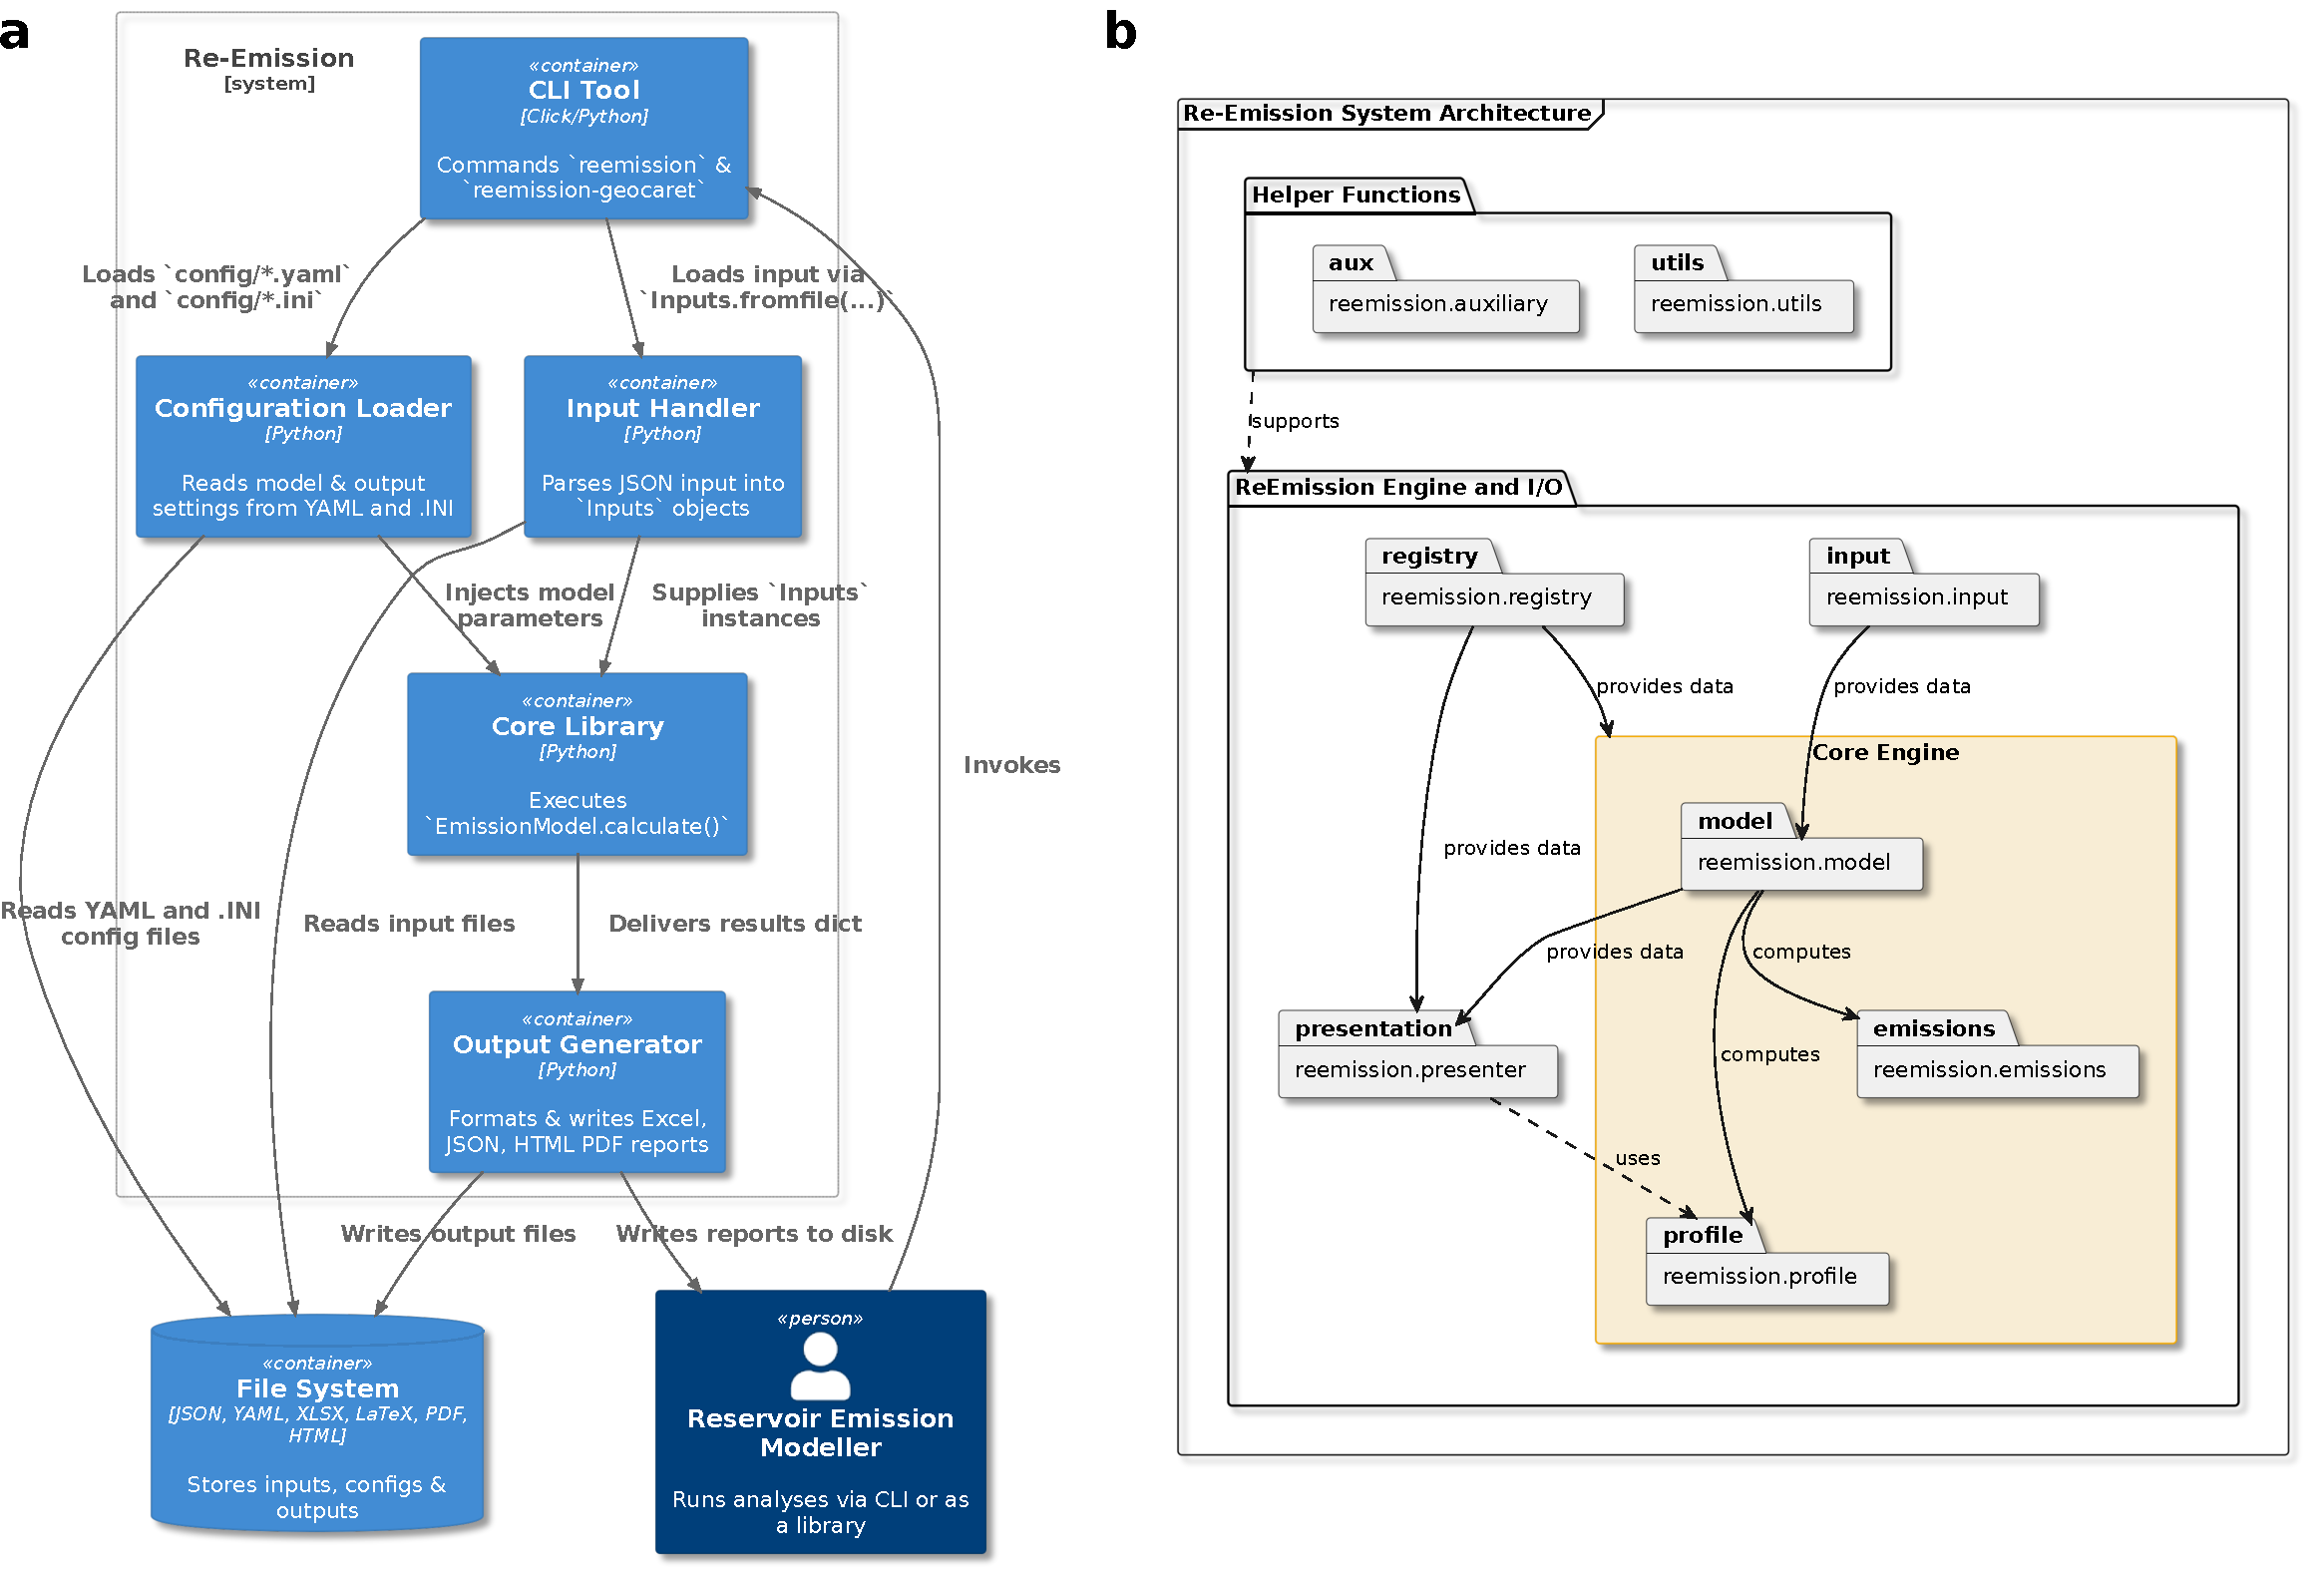
\includegraphics[width=0.99\textwidth]{figures/high_level_achitecture.pdf}
	\caption{Architecture of \textit{Re-Emission}. \textbf{a}, Container-level interactions showing key components, their functionalities, and data flow between system elements. Users can interact with the \acf{CLI} or Python library to load configuration parameters and input data, run the core emission models, and generate reports in multiple formats (Excel, JSON, PDF, HTML). Configuration files specify model parameters and presentation settings for the outputs, while the file system manages input and output storage. \textbf{b}, Package dependency view highlighting the modular structure and inter-package relationships within the system.}
    \label{fig:high_level_archtecture}
\end{figure}

The high-level architecture of the Re-Emission framework is illustrated in Figure~\ref{fig:high_level_archtecture}.
Re-Emission can be used either via a \acf{CLI} or by directly accessing its Core Library components within Python scripts, as shown in Figure~\figref[a]{fig:high_level_archtecture}.
The \ac{CLI} serves as the primary user interface, enabling emission analyses through straightforward commands.
When a command is executed, control is passed to a configuration loader, which parses and validates the user-defined model parameters, execution settings (e.g., selection of submodels), and presentation options (e.g., choice of output variables and associated metadata).
These configurations are specified in YAML and INI files located in the \vrbbrk{reemission/config/} directory and are then passed to both the Core Library and the \vrbbrk{reemission.presenter} module (Figure~\figref[b]{fig:high_level_archtecture}).
This design enforces a clear separation between logic (model equations) and data (parameters and inputs).

Input data are provided in JSON format and include reservoir, catchment, and climatic variables. 
These are read by \vrbbrk{reemission.input} and converted into a strongly typed \vrbbrk{Inputs} object used by the emission model.
Input data can be compiled manually from various data sources or generated automatically through upstream tools such as GeoCARET~\cite{heettool}, with which Re-Emission integrates (see Section~\ref{sec:integration}).
Upon completion of a model run, outputs are passed to a reporting engine that generates results in multiple formats, including Excel workbooks (XLSX), structured JSON files, as well as HTML and PDF reports.
Presentation functionality is handled by \vrbbrk{reemission.presenter}, which collates inputs, outputs, and intermediate variables from \vrbbrk{reemission.model} and \vrbbrk{reemission.profile}.
This enables both textual and graphical visualisations of the simulation outputs.
The loading, modification, and reuse of configuration files are managed by the \vrbbrk{reemission.registry} module.
%e cumulative reservoir emissions over time, based on each reservoirs' construction dates and their respective emission decay rates. 
% % -- such as regression coefficients, pre-impoundment emissions, and nutrient exports from land -- such as choice of submodels
%The input data and configuration settings are then routed into the Core Library highlighted in Figure~\figref[b]{fig:high_level_archtecture} by a lemon yellow rectangle. 
%The Core Library comprises the emission model, which runs the analysis using selected emission models and passes the results to \vrbbrk{reemission.presenter}. 

\begin{figure}[ht]
    \centering
    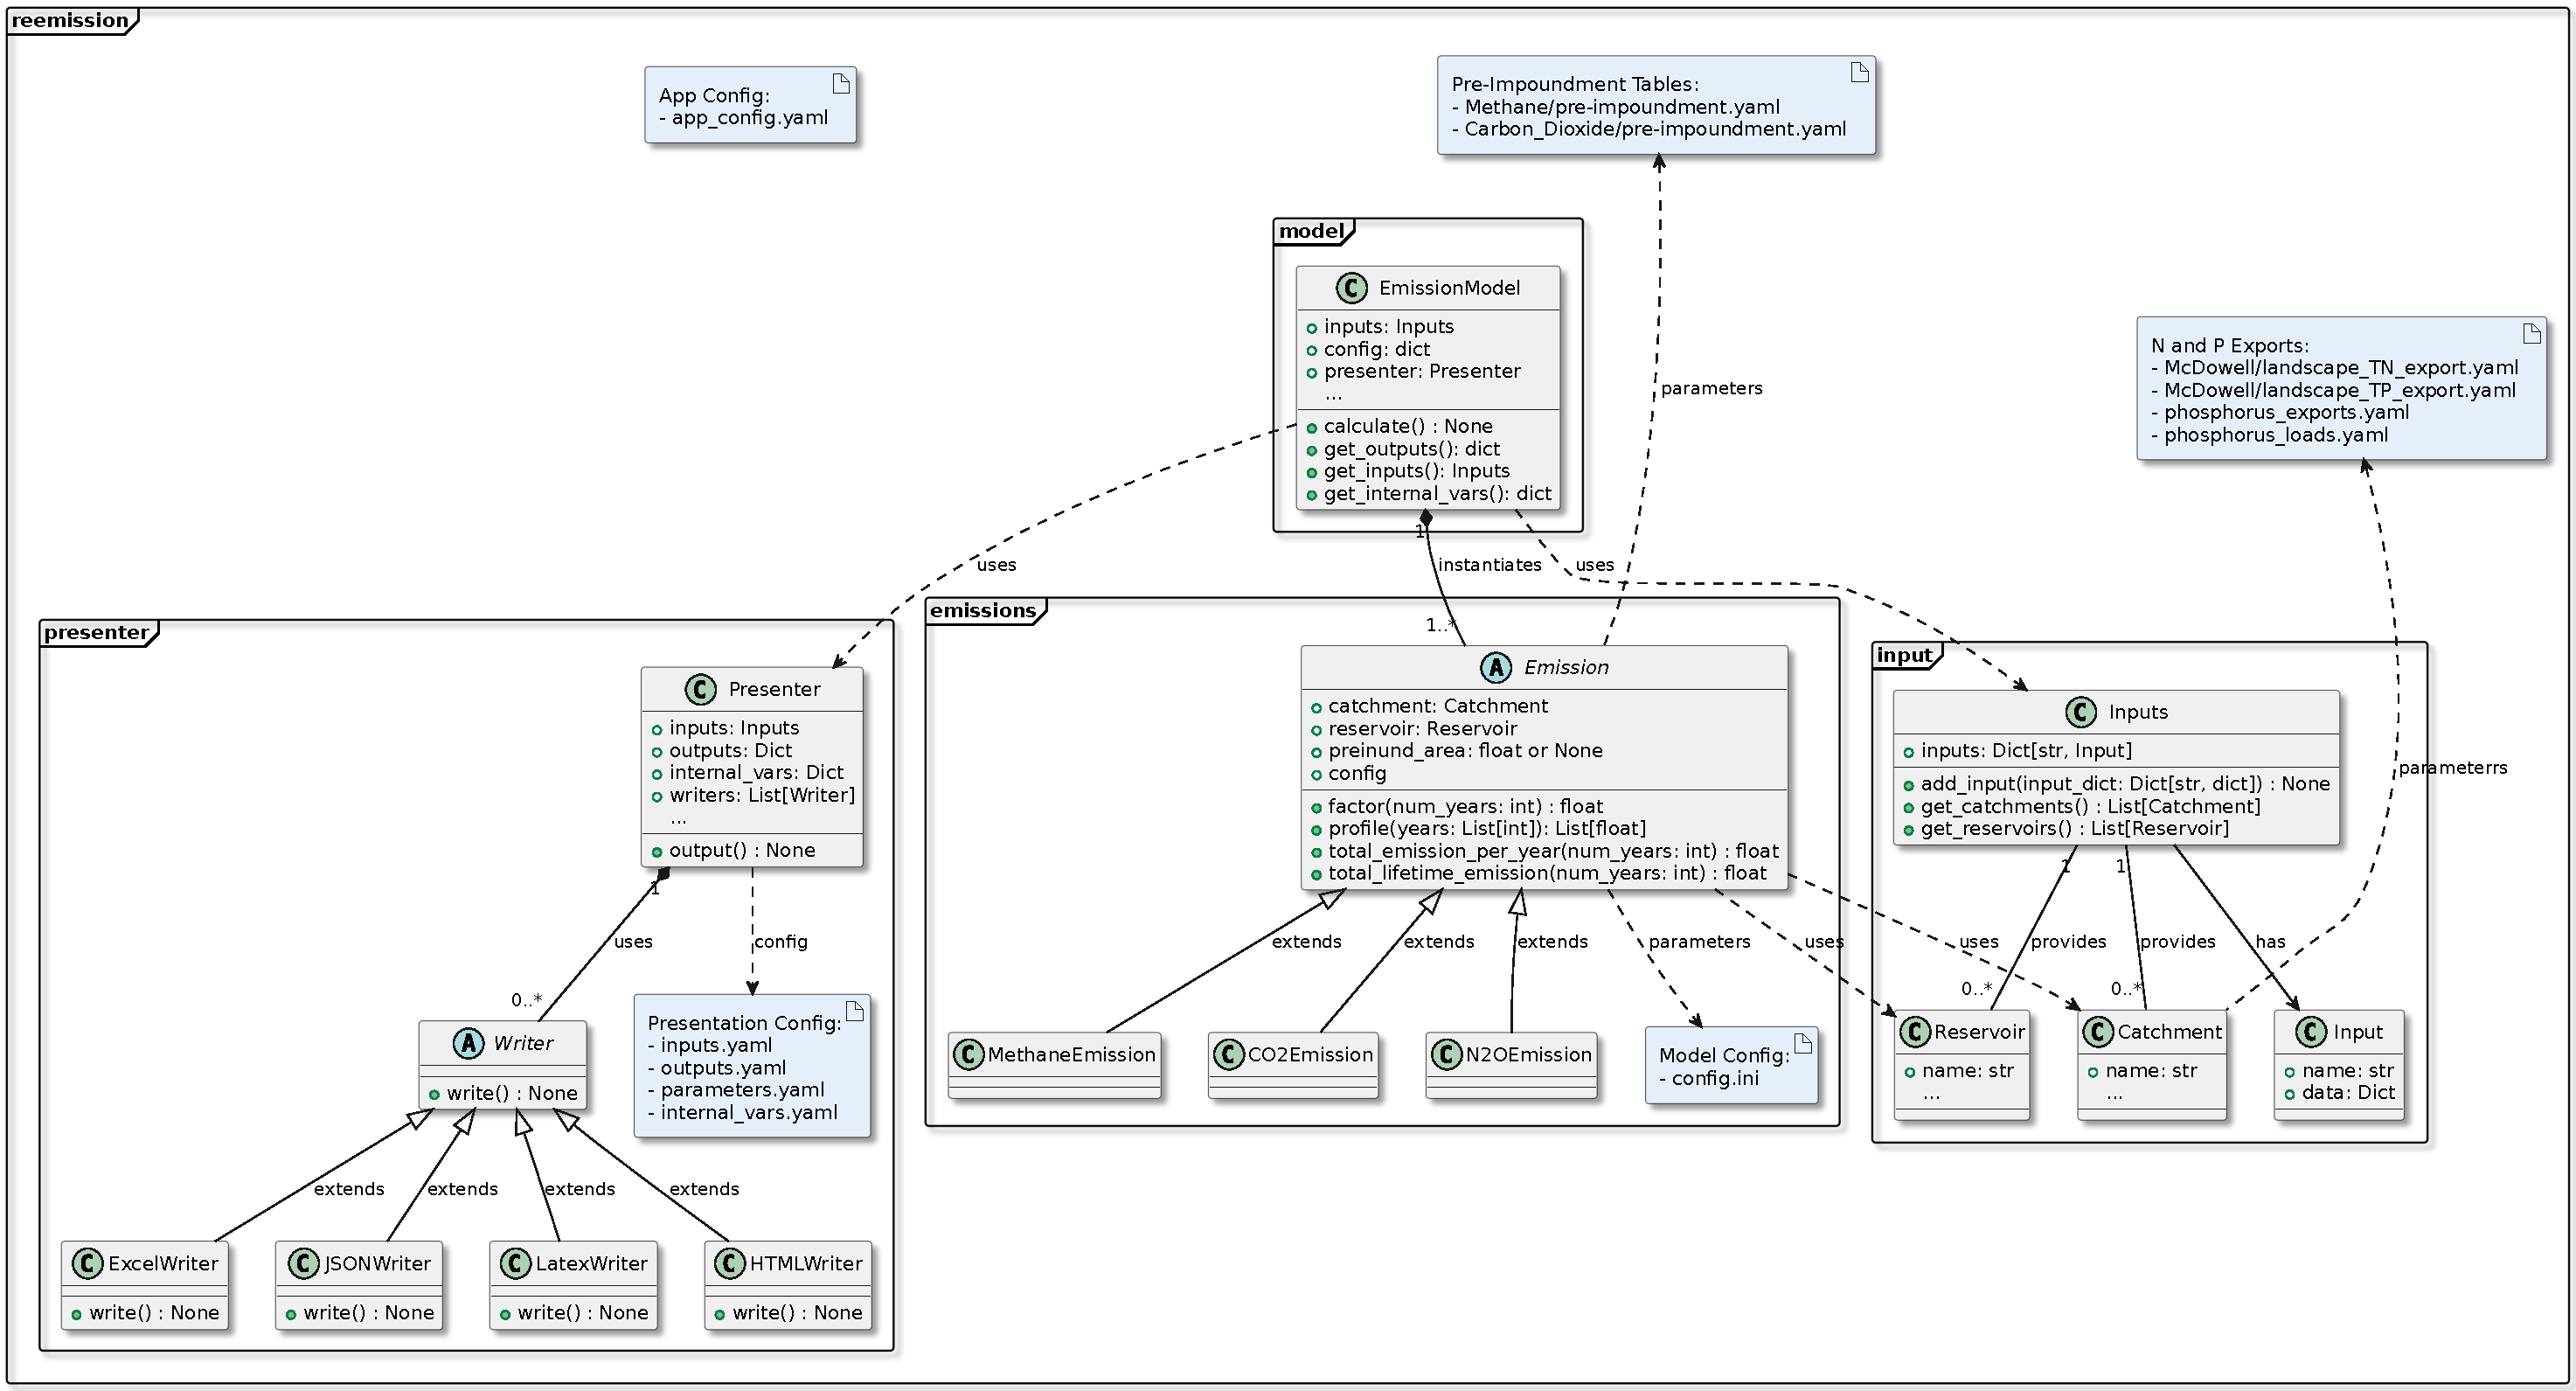
\includegraphics[width=0.99\textwidth]{figures/high_level_uml2.pdf}
	\caption{UML class diagram of \textit{Re-Emission}, illustrating key classes and their relationships. Core components include \texttt{EmissionModel}, \texttt{Reservoir}, \texttt{Catchment}, \texttt{Emission}, \texttt{Inputs}, and \texttt{Presenter}, with abstract interfaces used to enforce modularity and extensibility.}
    \label{fig:high_level_uml}
\end{figure}

A more detailed representation of the internal structure and inter-class relationships is shown in the UML class diagram in Figure~\ref{fig:high_level_uml}.
The \texttt{EmissionModel} class encapsulates the core simulation logic, including the instantiation of \vrbbrk{Reservoir}, \vrbbrk{Catchment}, and \vrbbrk{Emission} objects (e.g., \vrbbrk{MethaneEmission} for CH$_4$), and the subsequent computation of intermediate and output \ac{GHG} variables.
The \vrbbrk{Reservoir} and \vrbbrk{Catchment} objects are provided to the \vrbbrk{EmissionModel} via the \vrbbrk{Inputs} class.
Each \vrbbrk{Emission} object inherits from an abstract \vrbbrk{Emission} base class, which defines four abstract methods that must be implemented by all subclasses.
The \vrbbrk{Presenter} class uses \vrbbrk{Writer} objects to export outputs in different formats.
All \vrbbrk{Writer} objects inherit from an abstract \vrbbrk{Writer} base class that defines a unified interface for generating outputs.
Supported output formats include JSON, XLSX, PDF (via \LaTeX), and HTML.
The \vrbbrk{Reservoir}, \vrbbrk{Catchment}, \vrbbrk{Emission}, and \vrbbrk{Presenter} classes are parameterized via configuration files containing regression coefficients, pre-impoundment emission factors, nutrient export rates, and presentation options specific to the \vrbbrk{Presenter}.
Further details on the internal structure of the \vrbbrk{Reservoir} and \vrbbrk{Catchment} classes, as well as model input representations, are provided in the Appendix in Figure~\ref{fig:river_network_emissions_uml}.

\subsection{Using Re-Emission as a library}
\label{subsec:scripting}

Re-Emission can be used as a Python library, allowing its functions and classes to be invoked directly within Python scripts to perform emission calculations.
These calculations can be conducted step by step by manually constructing \vrbbrk{Reservoir} and \vrbbrk{Catchment} objects, followed by instantiating and executing \vrbbrk{Emission} objects, as demonstrated in Listings~\ref{lst:em_calc_setup} and~\ref{lst:em_calc} in the Appendix.
Alternatively, the \vrbbrk{EmissionModel} class provides a streamlined interface for this process, as illustrated in Listing~\ref{lst:em_calc_file}.
In addition to simplifying execution, use of the \vrbbrk{EmissionModel} class enables results to be exported in multiple formats via the \vrbbrk{Presenter} class (see Listing~\ref{lst:em_calc_presentation}).
In both modes of use, the analytical workflow, excluding result presentation, follows the algorithmic structure shown in Algorithm~\ref{alg:reemission}. Input data and model parameters are first read from structured data and configuration files. These inputs are then validated prior to computation. Emissions are subsequently calculated for each reservoir defined in the dataset, and raw results are saved to a JSON output file.

\begin{algorithm}[H]
\caption{Reservoir Emission Estimation}
\label{alg:reemission}
\SetKwInOut{Input}{Input}
\SetKwInOut{Output}{Output}

\AlgoDisplayBlockMarkers

\Input{Input file path (e.g., \texttt{input\_file.json})\\
       Configuration file path (e.g., \texttt{config\_file.yaml})}
\Output{Output file path (e.g., \texttt{output\_file.json})}

\BlankLine
Load input data from \texttt{input\_file.json}\;
\If{input is invalid}{
    Raise error and exit\;
}
Initialize model parameters from configuration file\;
\ForEach{entry in dataset}{
    Instantiate \texttt{Reservoir} and \texttt{Catchment} objects\;
    Instantiate \texttt{CarbonDioxideEmission} and \texttt{MethaneEmission} objects\;
    Estimate annual CO\textsubscript{2} and CH\textsubscript{4} fluxes and flux profiles\;
}
Save results to \texttt{output\_file.json}\;
\end{algorithm}


\subsection{Command-Line Interface}
\label{subsec:cli}

Re-Emission can also be used via a simple \acf{CLI}.
Full usage instructions are available by running \vrbbrk{reemission --help} in a terminal or console.
A typical command-line invocation is illustrated in Listing~\ref{lst:em_calc_cli}, where input data are supplied in \vrbbrk{input.json}, and outputs are generated in multiple formats, including PDF, JSON, XLSX, and HTML.
Beyond emission calculation, the \ac{CLI} also supports commands for converting and modifying input datasets.
These capabilities are described further in Section~\ref{sec:integration}, which focuses on integration with upstream reservoir and catchment data processing workflows (see also Listing~\ref{lst:integration_cli}).

\begin{minipage}{0.95\textwidth}
\begin{lstlisting}[language=bash, label={lst:em_calc_cli}, caption={Re-Emission \ac{CLI}: Emission calculations using input.json as the source of input data.}]
> reemission calculate 
    input.json
    -o output.pdf -o output.json -o output.xlsx  -o output.html
    --author "John Smith" 
    --title  "Reservoir Emissions Analysis"
\end{lstlisting}
\end{minipage}

\subsection{Input and output data formats}
\label{subsec:input_output_formats}

The structure of the input and output data is illustrated in Figures~\ref{fig:input_data_format} and~\ref{fig:output_data_format}, respectively.
The input format is fixed and determined by the parameter requirements of the \vrbbrk{Reservoir} and \vrbbrk{Catchment} classes.
In contrast, the structure of the output data is configurable via YAML configuration files.
To improve clarity and readability, the figures show only a representative subset of the full input and output content.
Where data has been truncated, omissions are marked using bold, light-blue text followed by an ellipsis (...).

\begin{figure}[ht]
    \centering
    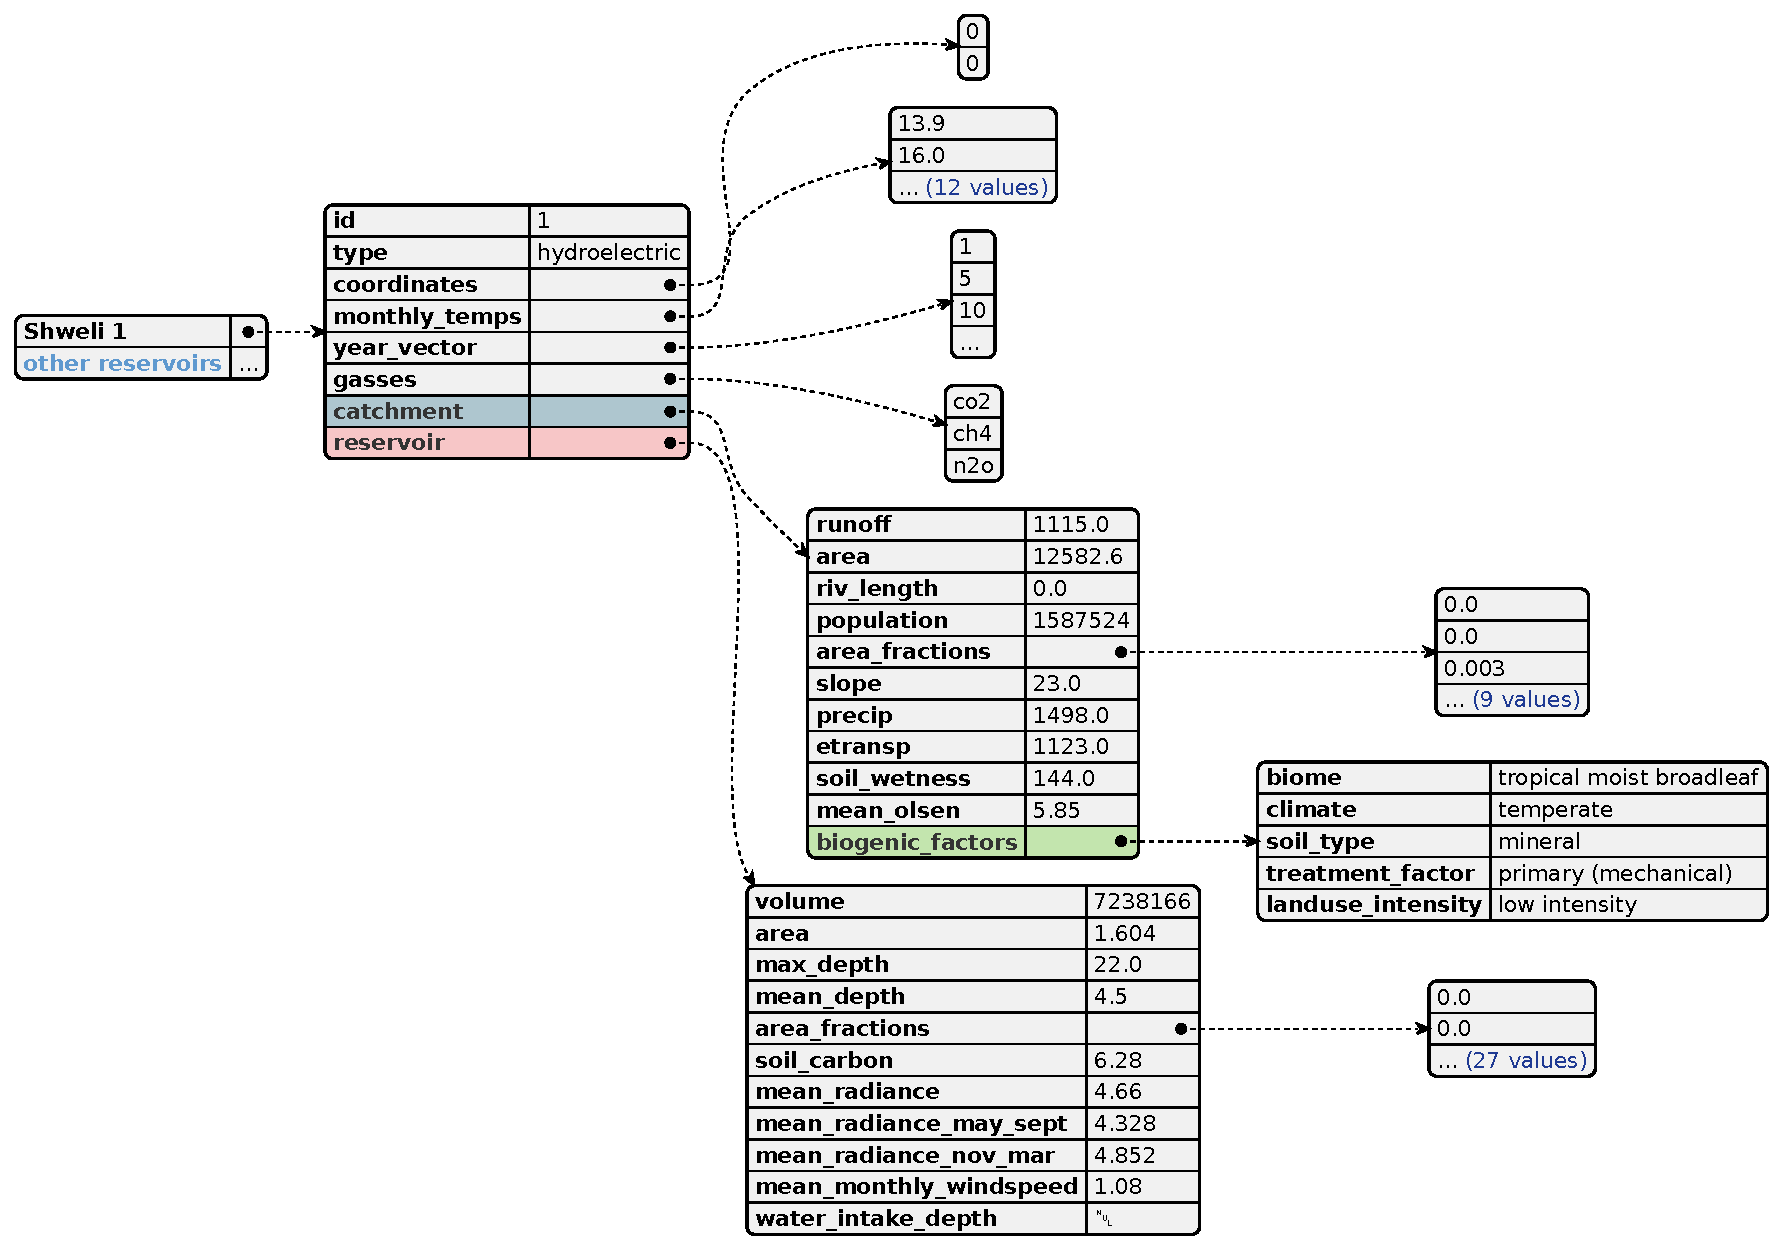
\includegraphics[width=0.75\textwidth]{figures/input_data_json.pdf}
    \caption{Structure of an input JSON file containing example data for a single reservoir. Entries related to catchment and reservoir parameters -- highlighted in steel blue and salmon, respectively -- correspond directly to fields defined in the \vrbbrk{Catchment} and \vrbbrk{Reservoir} classes. Selected values have been truncated for readability, with omissions indicated using light blue font colour followed by an ellipsis.}
    \label{fig:input_data_format}
\end{figure}

\begin{figure}[ht]
    \centering
    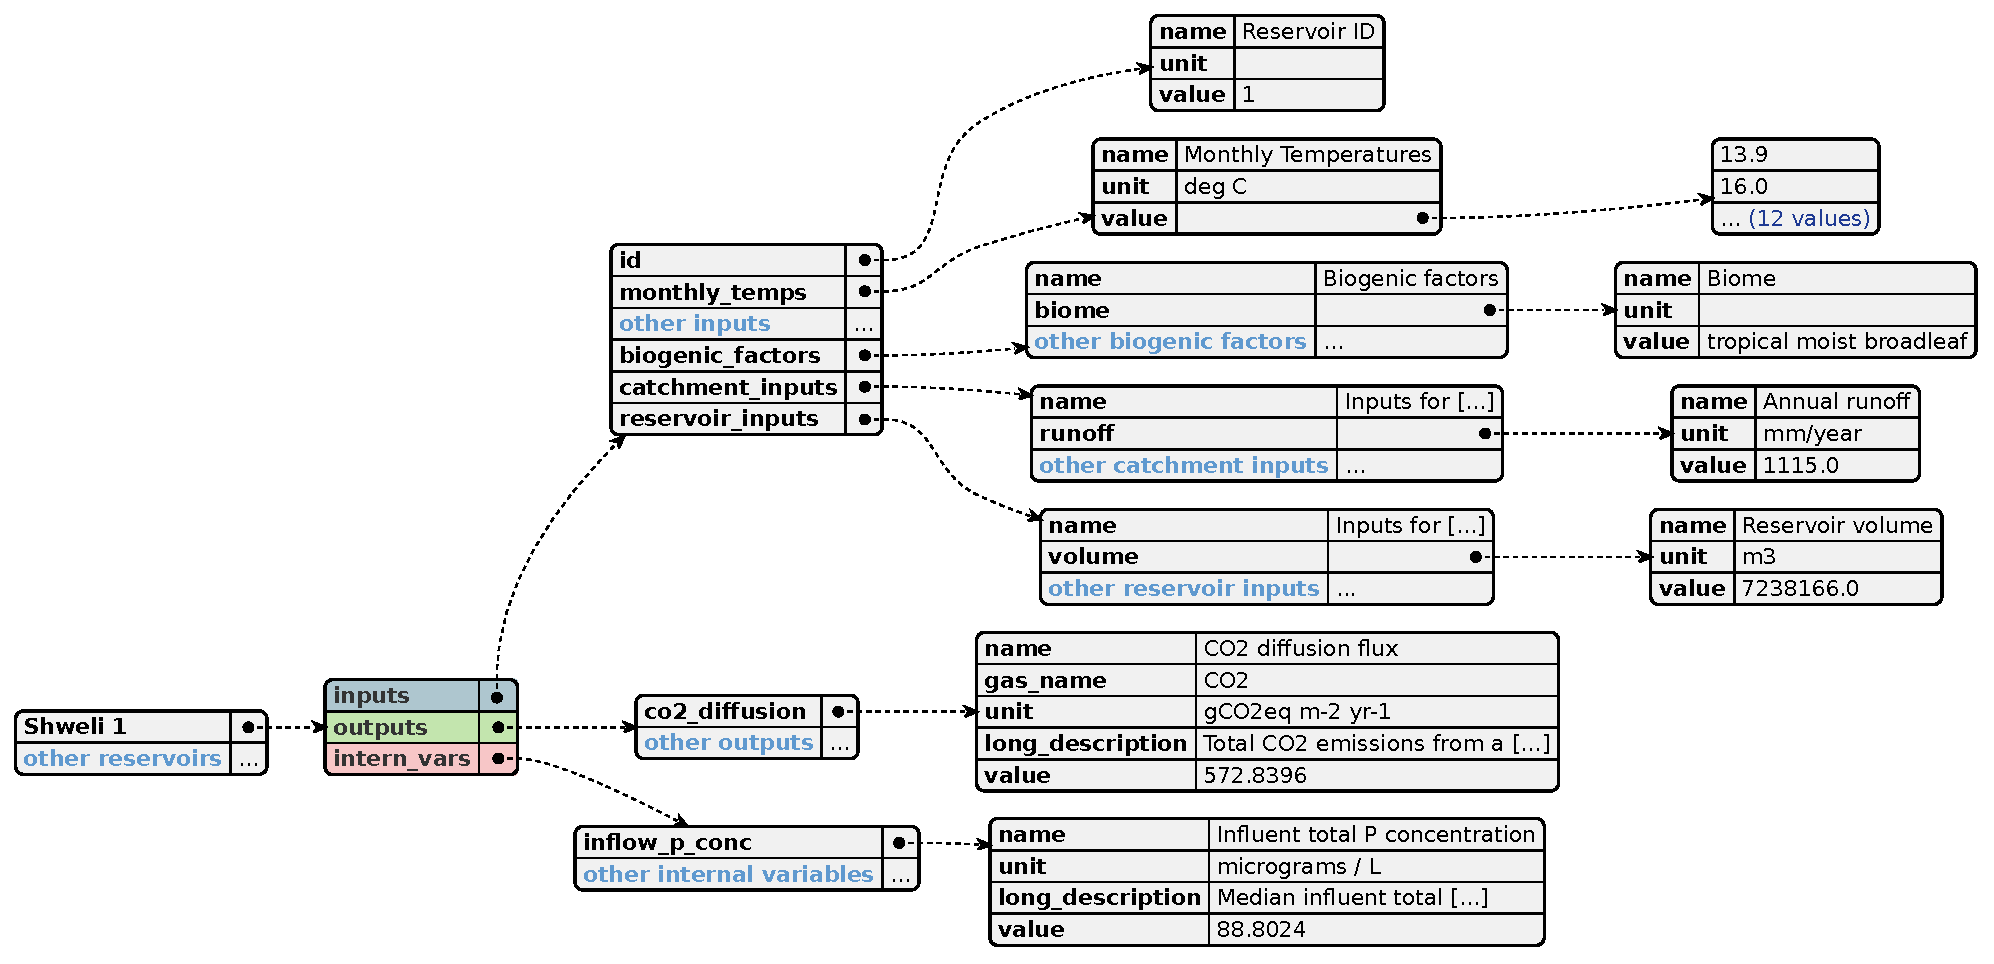
\includegraphics[width=0.9\textwidth]{figures/output_data_json.pdf}
    \caption{Structure of an example configurable output JSON file. The file is organized into three sections -- inputs, outputs, and internal variables -- highlighted in steel blue, olive green, and salmon, respectively. As the number of output entries can be arbitrarily large, selected values have been truncated for readability. Truncated content is indicated using light blue font colour followed by an ellipsis.}
    \label{fig:output_data_format}
\end{figure}

\subsection{Configuration options}
\label{subsec:config_options}

Configuration data -- including model parameters, options for the \vrbbrk{Presenter} class, and tabular inputs such as pre-impoundment emission factors or nutrient export coefficients -- is stored in INI and YAML files. 
These files provide semi-structured data representations that can be readily loaded into Python as dictionary objects.
The structure of these configuration files is illustrated in Figure~\ref{fig:config_uml} for presentation and model settings, Figure~\ref{fig:preimpoundment} for pre-impoundment emission factors, and Figure~\ref{fig:tp_tn_exports} for the parameterization of nutrient export models.

Configuration data is managed by the \vrbbrk{ConfigLoader} class, which registers configuration files and loads them lazily upon first access.
It also supports overriding default settings with user-defined configurations.
Instances of \vrbbrk{ConfigLoader} with registered configuration files are made globally accessible through the \vrbbrk{reemission.registry} module.

\subsection{Containerized execution using Docker}
\label{subsec:docker}

To ensure reproducibility and simplify the deployment of Re-Emission, we implemented a fully containerized workflow using Docker~\cite{merkel2014docker}, GitHub Actions, and the \acf{GHCR}, as illustrated in Figure~\ref{fig:docker_containerizing}.
This approach guarantees consistent runtime behaviour across computing environments and eliminates the need for complex setup procedures, thereby lowering the technical barrier to adoption.
Docker is an open-source platform that packages applications and their dependencies into standardized units called containers, which run in isolated environments.
Re-Emission, along with the Python interpreter, essential libraries, and other dependencies, is encapsulated in a Docker image.
The source code and Docker configuration files (e.g., \verb|compose.yaml|) are maintained in a GitHub repository, with \ac{CI} managed via GitHub Actions. Whenever changes are pushed to the \verb|release| branch, a Docker image is automatically built and published to the GitHub Container Registry.
This image can be retrieved using the standard \verb|docker pull| command, assuming Docker is installed on the user's machine.

The Re-Emission \ac{CLI} can be executed via \verb|docker compose run reemission| from a directory containing the appropriate \verb|compose.yaml| configuration file.
This file is required at runtime to map directories between the container and the host system, enabling access to input files and writing of output results.
To further streamline the Dockerized execution of Re-Emission, a companion repository is provided that defines the necessary folder structure, configuration files, and volume mappings for running the Re-Emission container~\cite{janus_geocaret_reemission}; see \emph{Software Availability}.

Currently, the shared Docker images for Re-Emission do not include a \LaTeX\ distribution, which is required for generating PDF reports via the \verb|pylatex| library.
This exclusion is deliberate, as bundling a full \LaTeX\ system -- such as TeXLive -- would significantly increase the image size, reducing portability and practicality for lightweight deployments.
Consequently, PDF report generation is not supported in the standard containerized version of Re-Emission.
However, equivalent HTML-based reports can be generated as described in Section\ref{subsec:input_output_formats}.
Users requiring PDF report generation within Docker must build a custom image by extending the official Re-Emission image with a \LaTeX\ installation.
This can be achieved by creating a new Dockerfile (see Listing~\ref{lst:docker_with_latex}) and building the image using the command \verb|docker build -t reemission-with-latex .| executed in the directory containing the Dockerfile.

\begin{figure}[ht]
    \centering
    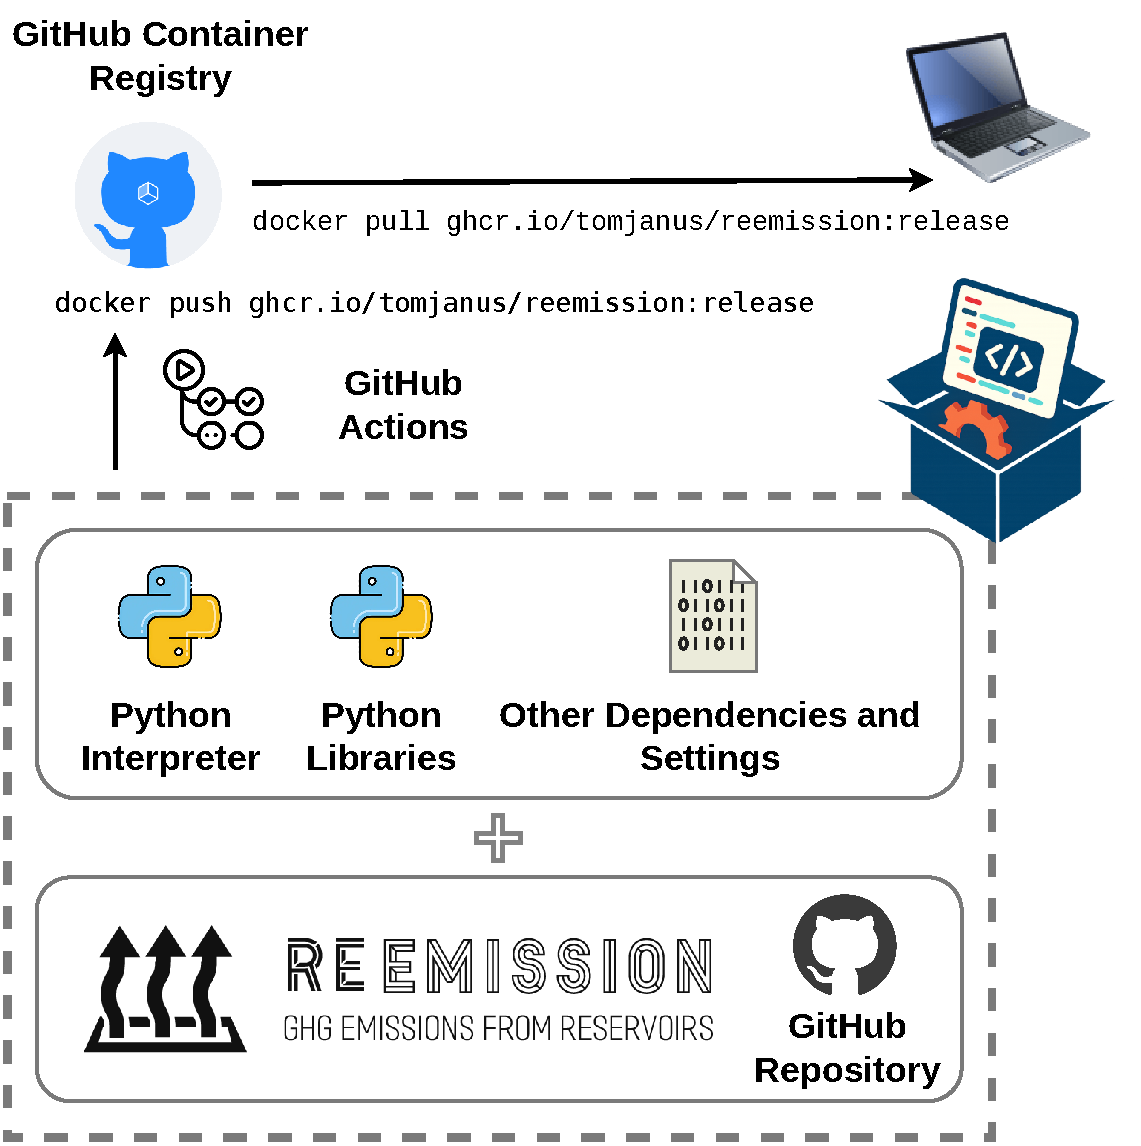
\includegraphics[width=0.55\textwidth]{figures/docker-explanation.drawio.pdf}
    \caption{{Containerized deployment of Re-Emission using Docker, GitHubActions, and the GitHub Container Registry.}}
    \label{fig:docker_containerizing}
\end{figure}

\begin{minipage}{0.95\textwidth}
\begin{lstlisting}[language=Dockerfile, , label={lst:docker_with_latex}, caption={Dockerfile for extending the Re-Emission image with a full TeX Live installation to support PDF report generation via PyLaTeX.}]
# Dockerfile
FROM ghcr.io/tomjanus/reemission:release
# Install TeX Live
RUN apt-get update && \
    apt-get install -y texlive-full && \
    apt-get clean && \
    rm -rf /var/lib/apt/lists/*
\end{lstlisting}
\end{minipage}

\section{Integration with upstream reservoir and catchment processing}
\label{sec:integration}

The principal challenge in estimating emissions from multiple reservoirs using spatially explicit emission models such as G-res lies in the manual effort and time required to source and derive the necessary input data.
When input variables are not directly available, they must be extracted from geospatial datasets using various \ac{GIS} methods.
This typically involves delineating each reservoir and its corresponding catchment area, followed by processing diverse datasets such as \acp{DEM}, land cover maps, soil and biome classification layers, and various climate-related datasets.
These steps are often labour-intensive and time-consuming, particularly at larger spatial scales.

To streamline this process, we provide functionality for generating input JSON files for Re-Emission from the outputs of the open-source Geospatial CAtchment and REservoir analysis Tool (GeoCARET)~\cite{heettool}.
GeoCARET defines algorithms for a variety of statistical and geometric operations required to derive reservoir and catchment characteristics, and executes them on \ac{GEE}~\cite{gorelick2017google} via its Python API.
This setup enables automated data acquisition and preprocessing across multiple reservoir sites with minimal overhead, supplying the necessary inputs for the G-res model.
Although GeoCARET is still in the early stages of development, it is already suitable for practical application and was used to generate the input data for the two case studies presented in this paper.

Integration between the tools is supported through a suite of \ac{CLI} functions, illustrated in Listing~\ref{lst:integration_cli}, that:
(i) merge multiple tabular files and populate missing variables (e.g., those not derivable from geospatial datasets and requiring manual input);
(ii) convert tabular data to JSON format; and
(iii) optionally merge individual reservoir and catchment shapefiles to support the mapping and visualization of emissions.
The integration workflow is further streamlined by running both tools within their respective Docker containers, coordinated through the Re-Emission--GeoCARET companion repository~\cite{janus_geocaret_reemission} introduced earlier (see \emph{Software Availability} for details).

\begin{minipage}{0.95\textwidth}
\begin{lstlisting}[language=bash, 
label={lst:integration_cli}, caption={Re-Emission CLI: Processing outputs from the GeoCARET reservoir and catchment processing tool.}]
# Step 1: Processing tabular GeoCARET outputs in multiple .csv files 
> reemission reemission-geocaret process-tab-outputs \
    -i  geocaret_outputs.csv \
    -o  reemission_inputs.csv \
    -cv 'c_treatment_factor' 'primary (mechanical)' \
    -cv 'c_landuse_intensity' 'low intensity' \
    -cv 'type' 'potable'
# Step 2: Creating Re-Emission input JSON file from the tabular CSV data
> reemission-geocaret tab-to-json 
    -i reemisison_inptus.csv 
    -o reemission_inputs.json
# Step 3: Merging shape files (one per individual reservoir, catchment, dam, etc.) into combined shapes per geometry type
> reemission-geocaret join-shapes \
    -i  input_folder
    -o  output_folder
    -gp 'R_*.shp, C_*.shp, PS_*.shp'
    -f  'reservoirs.shp, catchments.shp, dams.shp'
\end{lstlisting}
\end{minipage}

%% Use \subsubsection, \paragraph, \subparagraph commands to 
%% start 3rd, 4th and 5th level sections.
%% Refer following link for more details.
%% https://en.wikibooks.org/wiki/LaTeX/Document_Structure#Sectioning_commands

%% Refer following link for more details.
%% https://en.wikibooks.org/wiki/LaTeX/Floats,_Figures_and_Captions
%% https://en.wikibooks.org/wiki/LaTeX/Importing_Graphics#Importing_external_graphics

\section{Emission model validation}
\label{sec:validation}

We conducted a validation study to verify the correctness of Re-Emission's implementation of the G-res model and to ensure that no errors were introduced into the software’s core engine through the added complexity of presentation, input handling, and configuration modules.

To this end, we independently re-implemented the G-res model in the R programming language, following its original formulation~\cite{Prairie2021}.
Both implementations were used to compute final outputs -- such as gross and net areal CO$_2$ and CH$_4$ emissions across different emission pathways -- as well as intermediate variables involved in the emission calculations.
By systematically comparing outputs and inspecting the source code of both implementations, we substantially reduced the likelihood of computational discrepancies.

To assess model accuracy across a broad input space, we constructed a synthetic validation dataset by randomly perturbing categorical input variables.
This allowed us to explore parameter combinations not encountered in our case studies so far.
The resulting dataset comprises 246 reservoirs derived from modifications of real reservoirs located in Myanmar and the United Kingdom.
These inputs span a wide range of land-cover types, biomes, climate zones, soil types, land-use intensities, and catchment-wide treatment factors.

Agreement between Re-Emission and the R-based implementation is illustrated in Figures~\ref{fig:validation_plot_gross_emissions} and \ref{fig:validation_plot_net_emissions}.
The results show a near-perfect match across gross areal emissions by pathway (Figure~\ref{fig:validation_plot_gross_emissions}), pre-impoundment emissions (Figure~\figref[a]{fig:validation_plot_net_emissions}), and net anthropogenic emissions (Figure~\figref[b]{fig:validation_plot_net_emissions}), with coefficients of determination ($R^2$) equal to 1.000 in all cases.
These findings confirm that Re-Emission produces reliable estimates of reservoir emissions under a wide range of environmental and geographical conditions.

\begin{figure}[ht]
    \centering
    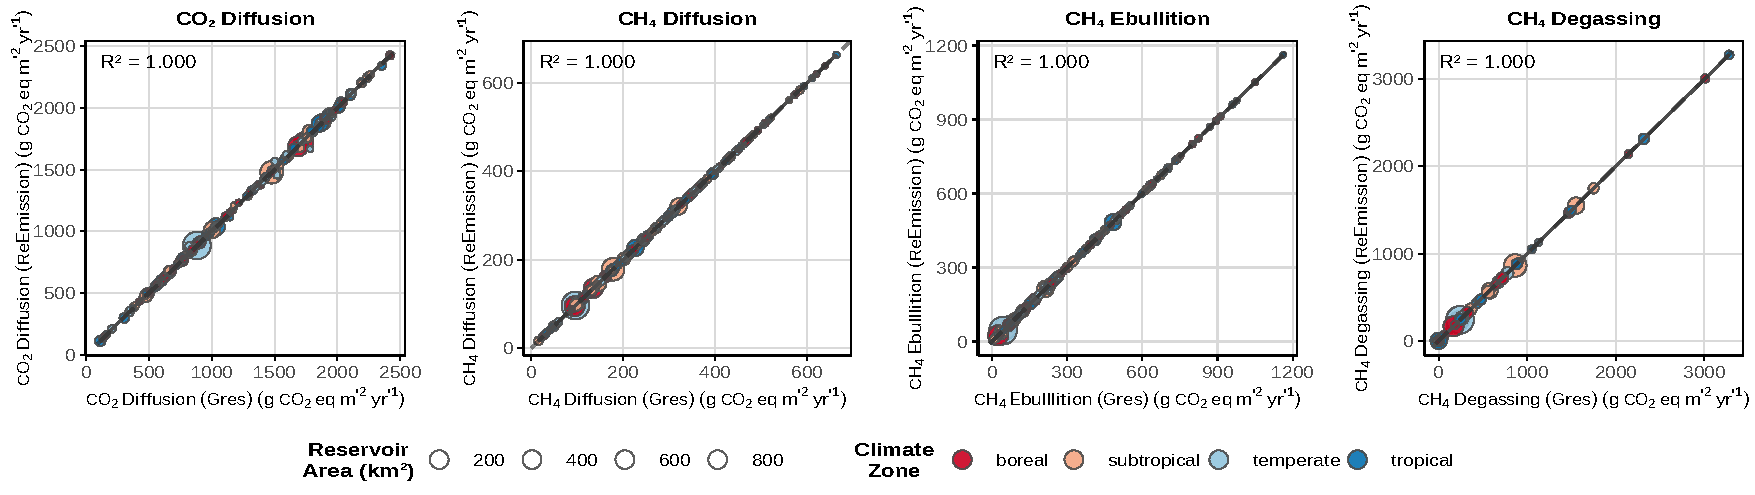
\includegraphics[width=1.0\textwidth]{figures/comparison_plot.pdf}
    \caption{{Comparison of gross areal emissions via four emission pathways -- CO$_2$ diffusion, CH$_4$ diffusion, CH$_4$ ebullition, and CH$_4$ degassing (from left to right) -- predicted using Re-Emission (y-axis) and the R-based G-res implementation (x-axis).}}
    \label{fig:validation_plot_gross_emissions}
\end{figure}

\begin{figure}[ht]
    \centering
    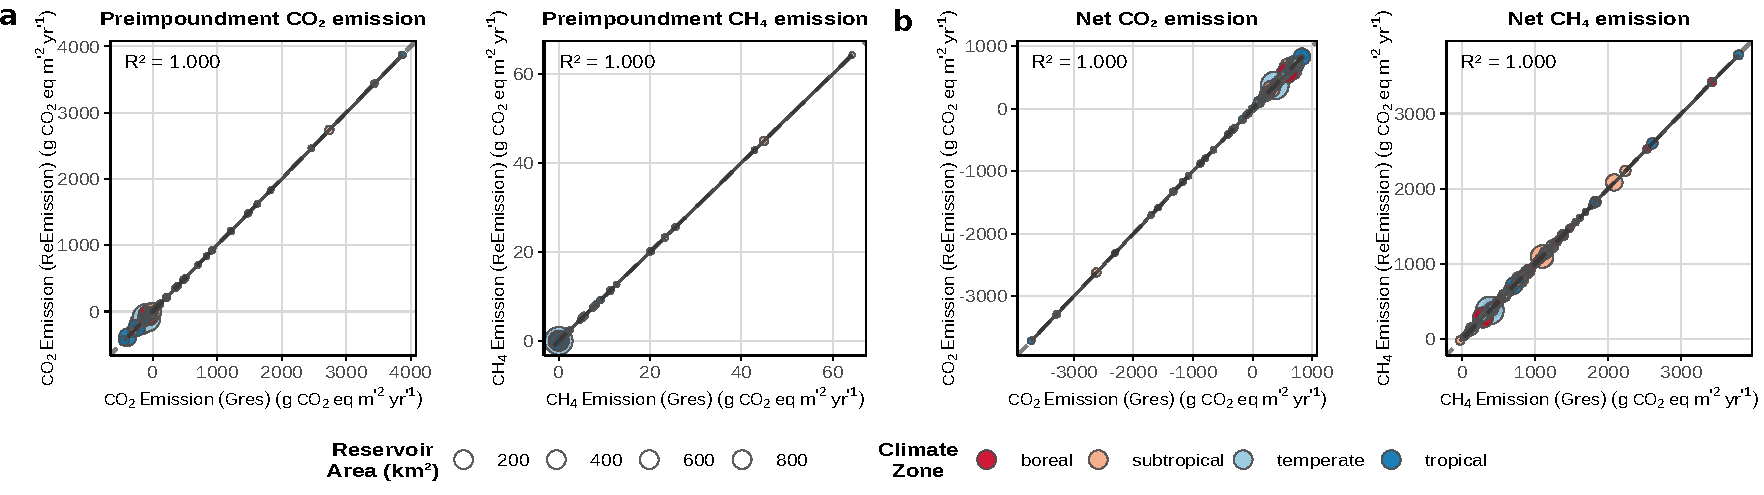
\includegraphics[width=1.0\textwidth]{figures/comparison_plot_net_emissions.pdf}
    \caption{{Comparison of (a) areal pre-impoundment CO$_2$ and CH$_4$ emissions and (b) net anthropogenic areal CO$_2$ and CH$_4$ emissions predicted using Re-Emission (y-axis) and the R-based G-res implementation (x-axis).}}
    
    \label{fig:validation_plot_net_emissions}
\end{figure}

\section{Case Studies}
\label{sec:case_studies}

We present two case studies to demonstrate key functionalities of Re-Emission for estimating \ac{GHG} emissions from reservoirs: (i) the estimation of total life-cycle emissions and emission profiles at scale, and (ii) the assessment of emissions under parametric uncertainty.
The first case study illustrates how Re-Emission facilitates emission assessments across multiple reservoirs, for example at regional or national scales. The second case study demonstrates the integration of Re-Emission with the Python-based sensitivity analysis library SALib~\cite{Iwanaga_Toward_SALib_2_0_2022}, enabling exploration of global sensitivity and uncertainty in emission predictions due to uncertain model parameters.
This functionality has both practical and scientific significance: it supports robust decision-making and contributes to methodological advancements in reservoir emission modelling.
To the best of our knowledge, the influence of uncertainties -- particularly input uncertainties -- on emission estimates has received limited attention in the existing literature.
Re-Emission helps address this gap by enabling uncertainty and sensitivity analysis of emission models with SALib.

\subsection{Emission trajectories from existing and planned assets in Myanmar}
\label{subsec:myanmar}

In this case study, we estimate the temporal evolution of total biogenic \ac{GHG} emissions and areal emission fluxes from more than 200 existing and planned reservoirs in Myanmar. 
Myanmar possesses substantial hydropower potential, with over 100~GW of identified capacity~\citep{EA_Myanmar}.
Although the country aims to triple its hydropower capacity by 2030~\citep{Aung2020}, the greenhouse gas implications of these proposed developments remain poorly understood. 
Moreover, biogenic emissions from existing irrigation reservoirs -- of which there are many -- have received limited attention despite their potentially significant atmospheric impact.

Using Re-Emission, we estimated emissions from all identified irrigation (IRR), multipurpose (MP), and hydropower (HP) reservoirs in Myanmar known to us. 
For each reservoir, we generated emission profiles (i.e., the temporal trajectory of biogenic emissions following impoundment) and aggregated them to derive national-scale emission trajectories.

Due to the lack of reliable construction date information for many reservoirs -- particularly existing irrigation schemes and proposed hydropower projects -- we employed a stochastic approach to scenario generation. 
Specifically, we constructed 1,000 plausible development scenarios by randomly sampling missing construction dates.
For each scenario, we simulated the temporal evolution of biogenic emissions from 1965 to 2045, thereby enabling an assessment of the timing and magnitude of peak emissions, as well as cumulative emissions over the planning horizon.
The missing construction dates for existing irrigation reservoirs were sampled from a \acf{KDE} fitted to a histogram of known construction dates.
This approach reflects historical trends in irrigation infrastructure development.
In contrast, the unknown commissioning dates for planned hydropower projects were sampled uniformly between the current year (2025) and an assumed planning horizon (2045), by which time all planned projects are assumed to become operational.

The results, presented in Figure~\ref{fig:mya_emission_profile}, show ensemble plots of possible emission trajectories, including the median profile and total emissions from irrigation reservoirs alone (IRR) as well as all reservoirs combined (IRR + HP + MP).
The findings suggest that uncertainty in the construction dates of irrigation reservoirs does not substantially affect the national emission profile for this class of assets. 
Emissions from these reservoirs appear to have peaked around 2005 and have been declining steadily since.
In contrast, the timing of construction for planned hydropower and multipurpose projects introduces significant uncertainty into the magnitude and timing of future emission peaks.
These projects are projected to contribute substantially to Myanmar’s biogenic \ac{GHG} emissions, with peak emissions likely to occur between 2030 and 2050.
While emissions are expected to decline sharply following the peak, they are projected to remain above current levels through at least 2060.

The insights provided by Figure~\ref{fig:mya_emission_profile} can inform national \ac{GHG} mitigation strategies and guide infrastructure planning.
With further extensions, the analytical framework demonstrated here could also incorporate other types of uncertainty -- such as model parameter uncertainty -- as described in the next case study.

\begin{figure}[ht]
    \centering
    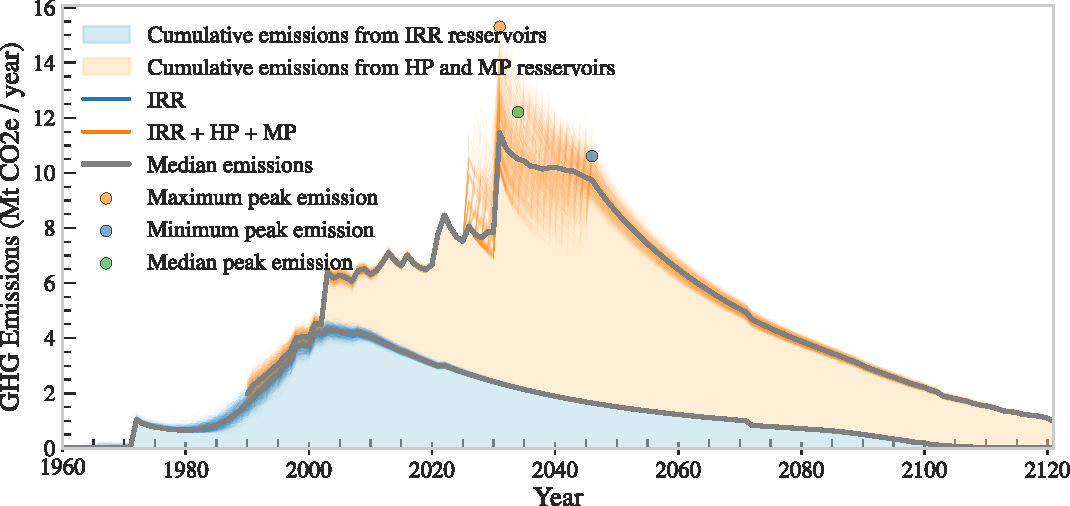
\includegraphics[width=0.8\textwidth]{figures/emission_profile.pdf}
    \caption{{Projected temporal evolution of emissions from existing and planned irrigation (IRR), multipurpose (MP), and hydroelectric (HP) reservoirs in Myanmar. In the absence of construction date information for some hydroelectric and multipurpose reservoirs, a 20-year planning horizon is assumed, by which all reservoirs included in current hydropower expansion plans are expected to be completed.}}
    \label{fig:mya_emission_profile}
\end{figure}

\subsection{Uncertainty analysis of reservoir emissions in Scotland and Wales}
\label{subsec:scotland_wales}

While it is widely acknowledged that emission model predictions are subject to considerable uncertainty, the magnitude and sources of these uncertainties remain poorly characterized. 
Reservoir emissions result from complex biogeochemical processes that are difficult to observe, model, and generalize due to their inherent spatio-temporal variability and often poorly understood dynamics.
Consequently, models developed from limited observational data may exhibit substantial epistemic and parametric uncertainties.
In addition, emission models typically rely on a large number of input variables -- many derived from geospatial datasets -- which themselves carry varying degrees of uncertainty.
These factors lead to compounded uncertainty in model outputs, with important implications for the reliability of emission estimates as a basis for decision-making and policy design.
Enabling uncertainty analysis and probabilistic emission estimation under parameter and input uncertainty is therefore of practical value to both researchers and practitioners.

Re-Emission facilitates the quantification of uncertainty arising from model parameters and inputs through an interface to the Python-based sensitivity analysis library SALib~\cite{Iwanaga_Toward_SALib_2_0_2022}.
At present, Re-Emission supports global sensitivity analysis using the Sobol method.
The interface leverages Re-Emission’s flexibility to dynamically modify configuration parameters -- such as regression coefficients for emission models, pre-impoundment emission factors, or nutrient export values -- to perform both sensitivity analysis and Monte Carlo simulations under parametric uncertainty.
It also supports uncertainty quantification arising from uncertain inputs and accommodates various probability distributions, including continuous, discrete, and categorical variables.

To demonstrate these capabilities, we conducted an analysis of parametric uncertainty in the G-res diffusive CO$_2$ and CH$_4$ emission models and evaluated their effect on total net anthropogenic emission estimates. 
This analysis was applied to 20 reservoirs located in Wales and Scotland. 
%The results are summarized in Figure~\ref{fig:uncertainty_analysis}. 
The results show that uncertainty in total net emission estimates is largely driven by the CO$_2$ diffusion process (Figure~\figref[b]{fig:uncertainty_analysis}), particularly the ``$\textrm{k}_1\,\textrm{diff}\,\textrm{co2}$'' coefficient. Coefficients ``$\textrm{k}_6\,\textrm{diff}\,\textrm{co2}$'' and ``$\textrm{k}_1\,\textrm{diff}\,\textrm{ch4}$'' also contribute to output variability, but their influence varies across reservoirs. This suggests that their importance is context-dependent, likely influenced by site-specific conditions or the relative contribution of individual emission pathways. 
Total net emission estimates for all 20 reservoirs, along with 95\% prediction intervals, are shown in Figure~\figref[c]{fig:uncertainty_analysis}.
The variability in prediction intervals across reservoirs is evident and again largely attributable to CO$_2$ diffusion uncertainty.
Figure~\figref[d]{fig:uncertainty_analysis} presents the probability density function of total net emissions for the Baddingsgill reservoir, illustrating the spread of values and indicating the mean, median, nominal estimate, and 5$^\textrm{th}$ and 95$^\textrm{th}$ percentiles.

Although this case study is intended for demonstration purposes, the approach can be readily extended to include additional parametric and input uncertainties -- both of which are supported by Re-Emission.
Due to the computational demands of Sobol analysis, however, expanding the number of uncertain parameters may require access to high-performance parallel computing environments.
Assessing reservoir emissions under uncertainty remains an open research area, and Re-Emission provides a flexible and extensible platform for advancing such analyses.

\begin{figure}[!h]
    \centering
    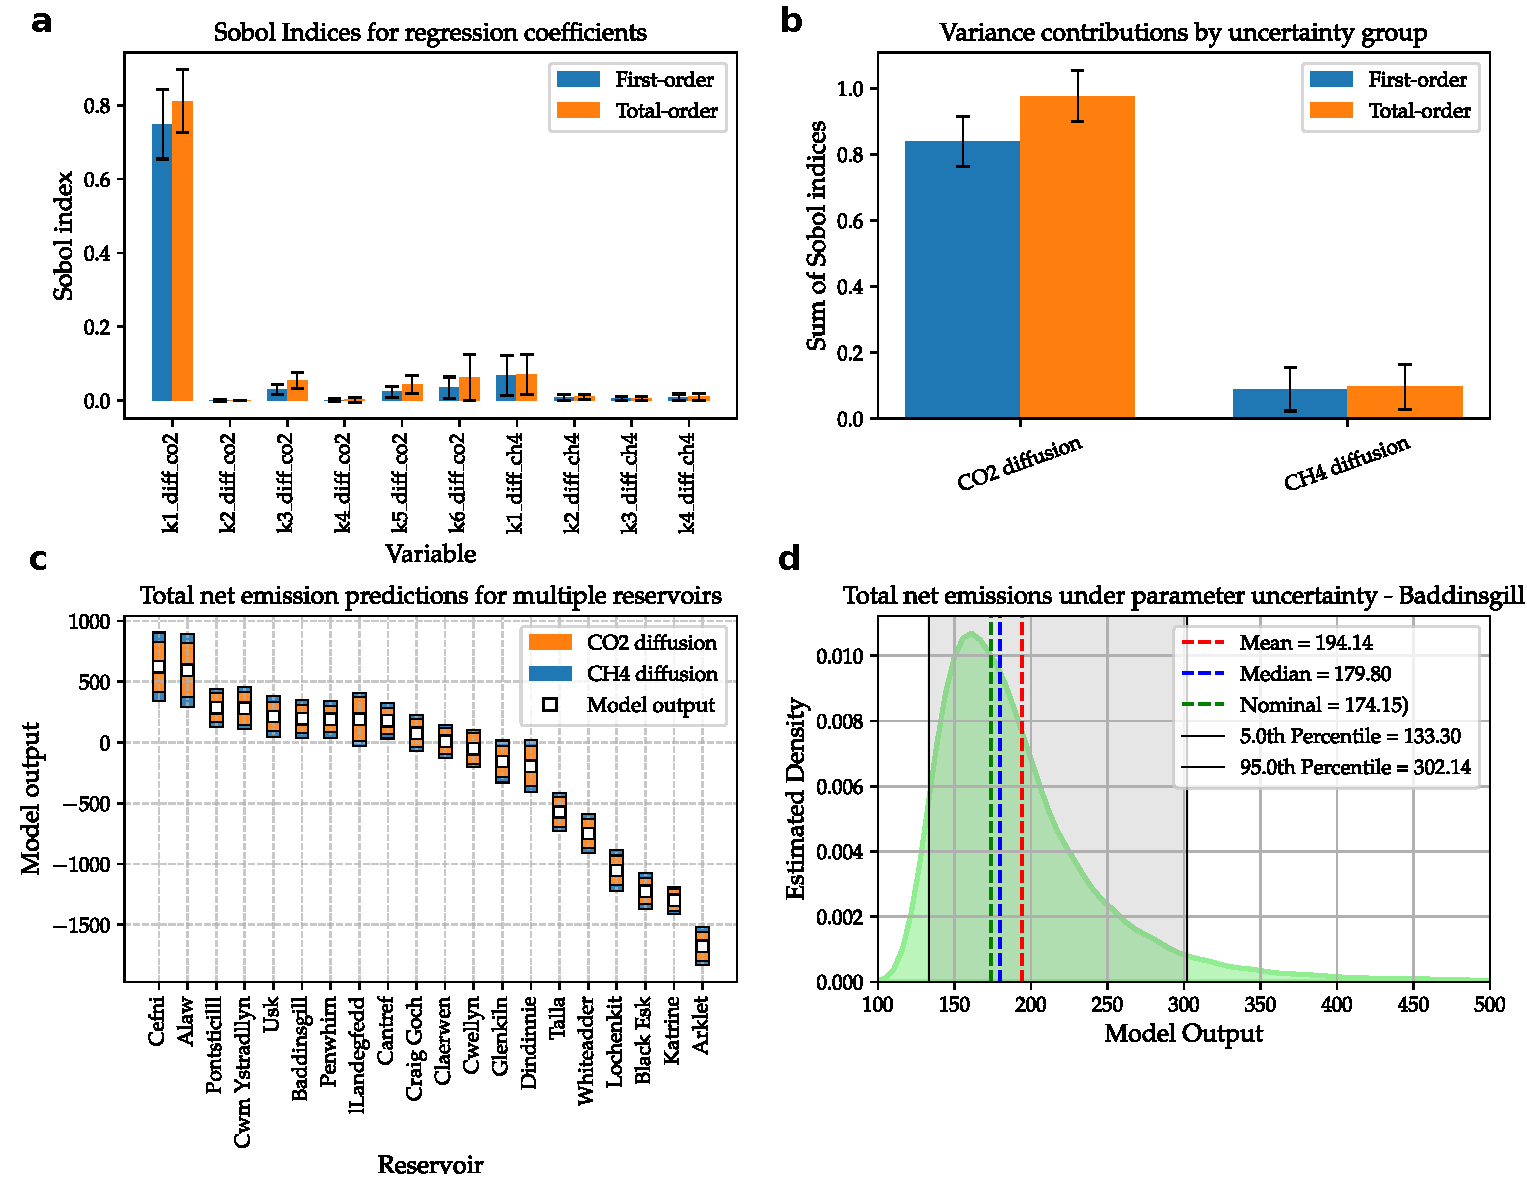
\includegraphics[width=1.0\textwidth]{figures/reemission_sobol_paper.pdf}
    \caption{
Quantification of parametric uncertainty in total net emissions from CO$_2$ and CH$_4$ diffusion processes for 20 reservoirs in Wales and Scotland. 
\textbf{(a)} First-order and total-order Sobol indices for the CO$_2$ and CH$_4$ diffusion regression coefficients, with error bars indicating variability across reservoirs. 
\textbf{(b)} Aggregated Sobol indices (first- and total-order) grouped by sources of uncertainty. 
\textbf{(c)} Total net emission estimates for the 20 reservoirs, with error bars indicating 95\% prediction intervals; the contribution of each uncertainty group is color-coded. 
\textbf{(d)} Probability density function of total net emissions for a selected reservoir, with mean, median, nominal values, and the 5$^\textrm{th}$ and 95$^\textrm{th}$ percentiles indicated.
}
    \label{fig:uncertainty_analysis}
\end{figure}


% ----- for information only ------
%The mineral/organic soil partitioning is derived from the ‘soil grids’ global layers, from which the soil C content is calculated as the mean C content of the inundated reservoir area and provided in the variable \verb|r_msocs_kgperm2|. It is required for distinguishing mineral from organic soils in the impounded/inundated reservoir area in order to apply correct \ac{IPCC} default tier1 ghg emission factors by climatezone and landcover type to estimate pre-impoundment GHG fluxes. 
%(seek definition) The organic soils are broadly peats that are positioned deeper than 40cm in the soil column and are thus somewhat restricted to specific areas (boreal, temperate uplands (Scotland), tropical uplands (andes) and basins (Congo) and SW Asia, such as Indonesia , with lots of palm on peat).
%(Chris) The general and \ac{IPCC} definition of organic soils (see image at end of this mail- I don’t find this free of ambiguity but anyway) is that they contain $>$12\% organic carbon by weight in the 0-30cm soil horizon.
%If 40 kg OC m-2 is expressed as a \% of soil volume (GRES text), with 1g OC incorrectly taken as = 1cm3 and 1cm3 soil = 1 g soil, for the 0-30cm strata, we get total mass or vol of soil in 0-30cm for 1m2 = 300kg or 300dm3 or 0.3 m3
%40 / 300 = 0.13 = 13.3\%  SOC – this is close to the threshold of 12\%   (although 36 kg m-2 would yield exactly 12\% by this approach).
%This is incorrect and indeed there are no global incidences of  $>$c.25 kg OC m-2 for the 0-30cm soil horizon. Aside from my speculation I cannot see how gres may have estimated the \% OC from the soil OC stock data (t/ha for 0-30cm), or how to consolidate their approach with the \ac{IPCC} org soil definition. 
%What we need to try to do to get correct soil classification among Min and Org soils:    derive \% SOC for 0-30cm.
% ----- for information only ------


\section{Discussion}
\label{sec:discussion}

In this manuscript, we have identified a critical gap in the current technological landscape that limits the ability of scientists and practitioners to estimate greenhouse gas emissions from reservoirs using spatially explicit models.
To address this, we developed an open-source software tool that integrates with GeoCARET -- an automated reservoir and catchment processing framework -- to enable automated assessments of reservoir emissions.
We demonstrated the software’s capabilities through two case studies, highlighting its application to large collections of reservoirs, its configurability, and its ability to support advanced analyses such as uncertainty quantification and probabilistic modelling.
While the tool represents a significant advancement over existing solutions, several limitations remain that warrant future development.
These limitations, along with the tool's benefits and proposed directions for further work, are discussed in the following sections.

\subsection{Limitations}
\label{subsec:limitations}

Despite its several advancements over existing software, Re-Emission currently exhibits notable limitations that warrant further development.
First, the tool is primarily designed to implement and extend the G-res model.
Consequently, it cannot be regarded as a general-purpose framework capable of accommodating a broad range of modelling paradigms (e.g., process-based approaches or hydrodynamic models).
Second, as Re-Emission incorporates the G-res model along with several of its extensions, it inherently inherits the limitations, biases, and uncertainties associated with these models.
%While the G-res model is largely based on the empirical dataset compiled by \citet{Deemer2016}—which includes measurements from 167 hydropower reservoirs globally—it suffers from uneven geographic representation. As a result, the regression-based relationships derived from this dataset may not adequately capture the diversity of reservoir types and climatic conditions, leading to potential biases and inaccuracies \citep[see, e.g.,][]{Hansen2022}.
Third, the current implementation does not support the simulation of emissions from cascading reservoir systems -- i.e., series of reservoirs where the outflow of an upstream reservoir forms the inflow to a downstream one.
This limits its applicability in river basins where such reservoir configurations are common.
Finally, Re-Emission is not yet equipped to integrate emission models for other aquatic systems, such as rivers and streams \citep{Rocher-Ros2023}, lakes \citep{Zhuang2023}, or wetlands \citep{Hu2024}.
Although modelling frameworks for these systems are still under development, future applications will likely require tools that enable multi-system integration.
Advancing towards integrated assessments of greenhouse gas and nutrient budgets at the catchment scale will be essential for generating more spatially resolved and transparent representations of aquatic system contributions to the global carbon cycle, thereby supporting science-based reporting and decision-making.

\subsection{Benefits}
\label{subsec:benefits}

The \emph{Re-Emission} package advances the state of the art in modelling reservoir \ac{GHG} emissions by providing a programmatic solution that supports batch processing and facilitates the scaling of emission assessments to multiple reservoirs.
In addition, it systematizes the modelling workflow for G-res and other prospective spatially explicit models that adopt similar conceptual frameworks. 
Its modular architecture and open-source nature allow users to extend the framework by incorporating new sub-models or applying custom parameterization, such as region-specific calibrations or updates based on new empirical data.
The importance of such model refinements and recalibrations has recently been emphasized by \citet{Pilla2025}.
Developed in Python -- one of the most widely used programming languages in scientific and engineering domains -- the tool can be seamlessly integrated into broader modelling pipelines.
This enables a wide range of applications, including the evaluation of emissions under parametric or input uncertainty, as well as integration with complementary tools such as GeoCARET for catchment and reservoir delineation, as demonstrated in this manuscript.
Finally, \emph{Re-Emission} provides a free and open-source alternative to proprietary solutions, offering cost-free emission analysis for both academic and commercial users.
Its transparent, modular, and automated design further promotes reproducibility and traceability in both research and applied contexts.

% ----- do not use this text ------
%designed to predict gross reservoir emissions via multiple emission pathways and quantify the share of net anthropogenic emissions
% and their underlying software is still limited.
%Overall, while the science of reservoir GHGs has advanced rapidly (from isolated measurements to global models), uncertainties are still large. Key research needs include more field data from underrepresented regions and reservoir types, better monitoring of all pathways (CH4, CO2, N2O), and refinement of predictive models (e.g. incorporating remote sensing of drawdown). In parallel, practitioners benefit from emerging tools: the G-res calculator and IPCC guidelines are widely used today, and new frameworks (e.g. automated geospatial models) are being developed to integrate GHG considerations into dam planning and policy.
%current ch4 measurements from Flooded Land are not sufficiently comprehensive to support the development of accurate default emission
%factors (especially for bubbles emissions and degassing emissions). 
%there is a lack of comprehensive data on the emission rates, dominant pathways and influence of various factors on emissions in reservoirs of different sizes, morphologies and locations. 
%The work is limited by the availability of data that cover a wide range of conditions in reservoirs  and identification of processes
%The significant share of reservoir emissions in global emissions combined with a growing reservoir storage globally (27.82$\pm$0.08~km$^3$/yr observed between 1999 and 2018~\cite{Li2023}) prompts for ...
% ----- do not use this text ------

\subsection{Future Work}
\label{subsec:future_work}

To address current limitations, future development of the Re-Emission framework will focus on enhancing modularity, interoperability, and flexibility to support next-generation assessments of reservoir \ac{GHG} emissions.
Although the current architecture is primarily centred on implementing the G-res model, we envision a transition to a network-based design that represents interconnected reservoirs and river reaches.
This structure would provide a more versatile foundation for modelling emissions from hydrologically connected water bodies and would overcome current limitations, such as the inability to represent cascading reservoir systems.
In this envisioned framework, carbon and nutrient mass balances would be explicitly solved, with emissions modelled as sinks, and inflows from river inlets and catchment runoff as sources.

Moreover, adopting a plugin-oriented architecture would allow for flexible model configurations by supporting interchangeable emission models and alternative formulations for key sub-processes, such as the estimation of hypolimnion depth or littoral zone area.
To enhance end-to-end automation and improve usability, tighter integration with upstream geospatial tools -- such as GeoCARET -- should be established to streamline the automatic sourcing and processing of catchment and reservoir input data.

Beyond architectural enhancements, future work must also address underrepresented emission pathways and processes.
Recent empirical studies have underscored the importance of previously unmodelled sources, such as methane emissions from sediments~\cite{gruca2011, Isidorova2019-ft} and downstream CH$_4$ degassing~\cite{Soued2022, Zhou2024}, which in some cases may account for up to 90\% of total reservoir-related emissions~\cite{Deshmukh}.
Accounting for these pathways will likely require coupling with complementary models or developing new modules that incorporate dynamic environmental conditions, including water level fluctuations and wetting-drying cycles in littoral zones~\cite{Calamita2021, Ion2021} -- necessitating a re-evaluation of existing modelling architectures.

Finally, although \acf{N2O} is a highly potent climate forcer, it remains the least studied of the three major \acp{GHG} in aquatic systems and is not yet routinely included in reservoir emission models.
However, global estimates suggest that lakes and reservoirs emit substantial amounts of N$_2$O~\cite{Li2024}, and recent studies indicate that under certain conditions -- particularly in nutrient-rich or thermally stratified systems -- N$_2$O emissions may rival or even exceed those of CH$_4$~\cite{Chen2025}.
These findings underscore the urgent need for expanded empirical observations and for the systematic integration of \ac{N2O} into reservoir modelling frameworks to more accurately represent the cumulative climatic impact of inland waters.


% ----- do not use this text ------
%A further area for exploration is the refinement of parameterizations related to nitrogen and phosphorus exports and pre-impoundment emissions, particularly for less-studied land-cover types such as wetlands or organic soils. For instance, land uses on peatlands or high-organic-content soils may exhibit distinct biogeochemical behaviour that is not currently captured in most empirical models.
%($\sim$65 Gg N$_2$O N yr$^{-1}$ in the 2010s), yet its inclusion in models remains rare. Recent studies suggest that N$_2$O emissions may rival or exceed CH$_4$ in specific contexts~\cite{Chen2025}, particularly in nutrient-rich or thermally stratified systems. These findings highlight the urgent need for additional empirical data and model integration to better represent N$_2$O dynamics within emission assessment tools.
%Collectively, these future directions will advance the \emph{Re-Emission} framework toward a comprehensive, extensible platform capable of supporting robust and policy-relevant emission modeling across scales and regions.
%To enhance end‐to‐end automation, we will improve interoperability with upstream geospatial analysis systems such as GeoCARET, enabling streamlined acquisition and formatting of catchment and reservoir input data. A common interface layer will be defined to standardize model input specifications, perform rigorous input validation, and manage metadata across diverse model components. This interface will facilitate the substitution of custom or third‐party data sources while ensuring consistency in variable naming, units, and quality control. Collectively, these enhancements will yield a more extensible, modular platform capable of supporting complex reservoir networks and diverse emission‐modeling strategies in large‐scale assessments.
%Recently, empirical studies addressed previously not researched emission mechanisms such as methane emissions from sediments~\cite{gruca2011, Isidorova2019-ft} and downstream CH$_4$ emissions~\cite{Soued2022} -- albeit the empirical models have not been formulated.
%larger groups of reservoirs for e.g. policy-making, country-wide emission assessments or integrating within larger planning studies, such as water, energy, food, etc.
%Experiment with parameterizations such as N and P exports and pre-impoundment emissions for less explored land-cover types, e.g. land uses on organic soils - \hl{give examples}
%Recent findings show that emission processes extend beyond reservoirs and can include downstream methane degassing~\cite{Zhou2024}, carbon peaking phenomena~\cite{Calamita2021}, and alterations in nutrient and organic matter fluxes that influence microbial processes and greenhouse gas production~\cite{Ion2021}. 
%In some cases, downstream emissions may account for up to 90\% of total reservoir-related emissions~\cite{Deshmukh}.
%Accurate modelling of these processes may require coupling with multiple complementary models or the adoption of more comprehensive frameworks that capture dynamic effects such as emissions driven by water level fluctuations or wetting-drying cycles in littoral zones.
%Unmeasured pathways are also a concern: as discussed above, drawdown-zone fluxes (CO2-dominated) were omitted in most studies, and nitrous oxide (N2O) -- a potent GHG -- has been sparsely measured. Recent analyses highlight that reservoirs and lakes are significant N2O emitters (globally ∼65 Gg N2O-N·yr-1 from lakes/reservoirs in 2010s
%From within three dominant gasses, N$_2$O emissions are least researched but may be significant under specific conditions, warranting further research, which results should be integrated into models and tools. 
%Modeling for Chinese dams suggests N2O may soon surpass CH4 in some contexts \cite{Chen2025}, underscoring a new knowledge need.  
% IPCC highlight considerable data gaps with respect to CH$_4$ emissions -- for example lack of emission data for major reservoir-bearing countries such as India, China and Russia. 
% ----- do not use this text ------

\section{Conclusions}
\label{sec:conclusions}

The \emph{Re-Emission} package represents a significant advancement toward standardized, transparent, and reproducible estimation of \acl{GHG} emissions from reservoirs.
By implementing the state-of-the-art G-Res model within an open-source Python environment, it provides researchers and practitioners with a flexible platform to apply, extend, and experiment with reservoir emission modelling across diverse contexts.
Integration with GeoCARET further enables automated emission estimation with minimal manual input, streamlining large-scale analyses of multiple reservoirs, as demonstrated in the two case studies presented.
Despite current limitations and the need for ongoing development, \emph{Re-Emission} is already suitable for practical applications, including emission assessments of individual reservoirs, regional and national infrastructure evaluations, and integration into more comprehensive analyses -- such as those supporting strategic planning in the \ac{WEFE} nexus.
Importantly, the development of this tool aligns with the recommendations of the \emph{2019 Refinement to the 2006 \acs{IPCC} Guidelines for National Greenhouse Gas Inventories: Wetlands}\cite{IPCC2019}, which advocate the adoption of Tier~2 or Tier~3 methodologies, such as G-Res, to reduce uncertainties in emission estimates where sufficient data and analytical capacity are available.

%Building on the foundations of the G-res model, this study proposes an enhanced approach that requires minimal input data. By using only the location and height of a proposed hydropower dam, a suite of hydro-morphological parameters describing the catchment and reservoir can be derived. These parameters are then employed to estimate \ac{GHG} emission trajectories over a 100-year period, leveraging empirical relationships between physical characteristics and emission rates. This approach enables rapid, spatially explicit assessments of potential reservoir emissions and supports strategic planning in dam development and climate impact mitigation.

%- The paper emphasizes the need for integrated modelling approaches that combine empirical data with mechanistic understanding to improve the accuracy of \ac{GHG} emission estimates~\citet{Zhao2021}  
%Despite of over two decades of research, 
%The community would benefit from having an open-source tool for experimenting with new models, model refinement, calibration to new data, etc.

% ------------------------
%While such methods allow estimating emissions from multiple reservoirs with minimal overhead, they were found to introduce significant biases and inaccuracies, especially for reservoirs with unique properties that fell outside the range of observed data~\cite{Harrison2021}. 
%located only in specific regions in the world and of certain morphological characteristics that are not representative of 
%In place of directly calculated values, recent studies on global reservoir emission assessments~\cite{Barros2011, Deemer2016, Harrison2021, Soued2022} and reservoir investment planning~\cite{Almeida2019, Flecker2022, Carlino2024} . 
%Yet there are limited studies \citep{Almeida2019, Soued2022} that detail emissions from future dams which is based on averaged emission rates per unit of surface area that rely on limited number of empirical studies.
%Apply these emission factors to assess emissions from future reservoirs~\cite{Almeida2019, Flecker2022, Tangi2024, Carlino2024}
%Reliable estimation of reservoir emissions is essential for understanding their current and potential future impacts on the global climate, and requires accurate models and scalable tools capable of assessing emissions across large ensembles of reservoirs.

\section{Software availability}
\label{sec:software_availability}
This paper describes the software in its current state of development, including all UML diagrams, code listings, and results. All such materials correspond to specific versions of the source code: commit \texttt{93944bd} for Re-Emission and commit \texttt{30a0796} for the Re-Emission–GeoCARET integration (see detailed information about both packages below).
The manuscript source files in \LaTeX, including all figures, as well as the Python and R scripts used to generate the case study results and validation plots, are available at \href{https://github.com/tomjanus/reemission-paper}{https://github.com/tomjanus/reemission-paper}.
In addition, the repository, along with all intermediate and final outputs, is archived on Zenodo at \href{https://doi.org/10.5281/zenodo.16424011}{doi:10.5281/zenodo.16424011}.

\begin{description}
  \item[\textbf{Name of the software:}] \texttt{Re-Emission}
  \item[\textbf{Developers:}] Tomasz Janus
  \item[\textbf{Contact address:}] \href{mailto:tomasz.janus@manchester.ac.uk}{tomasz.janus@manchester.ac.uk}, \href{mailto:tomasz.k.janus@gmail.com}{tomasz.k.janus@gmail.com}
  \item[\textbf{Year first available:}] 2022
  \item[\textbf{Hardware required:}] Windows 7, 10 (tested), 11, Linux (tested on Ubuntu 22.04), MacOSX
  \item[\textbf{Software required:}] \LaTeX \, (optional)
  \item[\textbf{Program language:}] Python 3.10+
  \item[\textbf{License:}] GNU General Public Licence v3
  \item[\textbf{Availability and cost:}] free and open source
  \item[\textbf{Source code:}] \href{https://github.com/tomjanus/reemission}{https://github.com/tomjanus/reemission} %and \href{https://pypi.org/project/pyclmuapp}{PyPI}
  \item[\textbf{Package:}] \href{https://github.com/tomjanus/reemission/pkgs/container/reemission}{https://github.com/tomjanus/reemission/pkgs/container/reemission}
  %\item[\textbf{Distribution:}] \hl{Put on PyPi and maybe also on conda-forge if straightforward to do - in case we do both, add two entries: Distribution (PyPi) and Distribution (conda-forge)}
  \item[\textbf{Documentation:}] \href{https://tomjanus.github.io/reemission}{https://tomjanus.github.io/reemission}
\end{description}

\vspace{3pt}

\begin{description}
  \item[\textbf{Name of the software:}] \texttt{Re-Emission GeoCARET Integration}
  \item[\textbf{Developers:}] Tomasz Janus
  \item[\textbf{Contact address:}] \href{mailto:tomasz.janus@manchester.ac.uk}{tomasz.janus@manchester.ac.uk}, \href{mailto:tomasz.k.janus@gmail.com}{tomasz.k.janus@gmail.com}
  \item[\textbf{Year first available:}] 2024
  \item[\textbf{Hardware required:}] Platform-independent
  \item[\textbf{Software required:}] Docker, \LaTeX \, (optional)
  \item[\textbf{Program language:}] YAML configuration
  \item[\textbf{License:}] GNU General Public Licence v3
  \item[\textbf{Availability and cost:}] free and open source, requires Google Earth Engine and Google Cloud registrations
  \item[\textbf{Source code:}] \href{https://github.com/tomjanus/geocaret-reemission}{https://github.com/tomjanus/geocaret-reemission}
  \item[\textbf{Packages:}] \href{https://github.com/tomjanus/reemission/pkgs/container/reemission}{https://github.com/tomjanus/reemission/pkgs/container/reemission}
\end{description}

\section{Declaration of competing interest}
The authors declare that they have no known competing financial interests or personal relationships that could have appeared to influence the work reported in this paper.

\section{Acknowledgements}
The authors would like to acknowledge the assistance provided by the Research IT Group at the University of Manchester, in particular James Sinnott, for their help in containerizing our software using Docker.
The development of the methodology and of the early version of Re-Emission and the Myanmar case study was supported by the UK Economic and Social Research Council's Global Challenges Research Fund (GCRF) as part of the UK Research and Innovation (UKRI) Funded FutureDAMS project(\href{www.futuredams.org}{ES/P011373/1}).
Work on containerising Re-Emission and Re-Emission GeoCARET integration was partially funded by UoM's Open Research Accelerator fund.
The case study on emission uncertainty quantification for UK reservoirs was funded by UoM's Policy@Manchester fund.
Further funding for T.J., J.K.and X.Z. was provided by their institutions. 
The work of C.B. was supported by the UK Centre for Ecology and Hydrology (UKCEH). 
Any opinions, findings, and conclusions or recommendations expressed in this material are those of the authors but not necessarily the funders.

%% The Appendices part is started with the command \appendix;
%% appendix sections are then done as normal sections
\appendix

\section{Selected Code Listings}
\label{app1}

\begin{minipage}{\textwidth}
\begin{lstlisting}[language=PythonReemission, label={lst:em_calc_setup}, caption={Use of Re-Emission as a library: step-by-step problem formulation.}]
from reemission.temperature import MonthlyTemperature
from reemission.emissions   import CarbonDioxideEmission, NitrousOxideEmission, MethaneEmission
from reemission.constants   import Landuse, Climate, SoilType, Biome, TreatmentFactor, LanduseIntensity
from reemission.catchment   import Catchment
from reemission.reservoir   import Reservoir
from reemission.biogenic    import BiogenicFactors

mt = MonthlyTemperature(
  [10.56,11.99,15.46,18.29,20.79,22.09,
   22.46,22.66,21.93,19.33,15.03,11.66])
coordinates = [22.6, 94.7] # Latitude and Longitude
biogenic_factors    = BiogenicFactors(
  biome             = Biome.TROPICALMOISTBROADLEAF,
  climate           = Climate.TROPICAL,
  soil_type         = SoilType.MINERAL,
  treatment_factor  = TreatmentFactor.NONE,
  landuse_intensity = LanduseIntensity.LOW)
catchment_area_fractions = \
  [0.0, 0.0, 0.0, 0.0, 0.0, 0.01092, 0.11996, 0.867257, 0.0]
reservoir_area_fractions = [
  0.0, 0.0, 0.0, 0.0, 0.0, 0.45, 0.15, 0.4, 0.0, 
  0.0, 0.0, 0.0, 0.0, 0.0, 0.0,  0.0,  0.0, 0.0, 
  0.0, 0.0, 0.0, 0.0, 0.0, 0.0,  0.0,  0.0, 0.0]
catchment_inputs = {
  'runoff'     : 1685.6, 'area'         : 78203, 'population' : 8463, 
  'riv_length' : 9.2,    'slope'        : 8.0,   'precip'     : 2000,   
  'etransp'    : 400,    'soil_wetness' : 140,   'mean_olsen' : 5.85, 
  'biogenic_factors' : biogenic_factors,
  'area_fractions'   : catchment_area_fractions}
reservoir_inputs = {
  'volume'       : 7.66E6, 'area': 100.6,       'max_depth'         : 32.0, 
  'mean_depth'   : 13.6,   'soil_carbon': 10.2, 'water_intake_depth': 20.0
  'mean_radiance': 4.5,    
  'mean_monthly_windspeed': 3.8, 'mean_radiance_may_sept': 4.5, 
  'mean_radiance_nov_mar' : 3.2, 'area_fractions': reservoir_area_fractions
}    
year_profile = (1, 5, 10, 20, 30, 40, 50, 65, 80, 100)
catchment = Catchment(**catchment_inputs)
reservoir = Reservoir(
  **reservoir_inputs,        temperature = mt,
  coordinates = coordinates, inflow_rate = catchment_1.discharge)
\end{lstlisting}
\end{minipage}

\begin{minipage}{\linewidth}
\begin{lstlisting}[language=PythonReemission, label={lst:em_calc}, caption={Use of Re-Emission as a library: calculation of CO$_2$ and CH$_4$ emissions using \texttt{CarbonDioxideEmission} and \texttt{MethaneEmission} classes.}]
em_co2 = CarbonDioxideEmission(
  catchment = catchment_1,            reservoir     = reservoir_1,
  eff_temp  = mt.eff_temp(gas='co2'), p_calc_method = 'g-res')
co2_emission_profile = em_co2.profile(years = year_profile)
co2_emission_factor  = em_co2.factor()    # Gross emission flux
co2_net_total        = em_co2.net_total() # Net anthropogenic emission flux
em_ch4 = MethaneEmission(
	catchment = catchment_1, reservoir = reservoir_1, monthly_temp = mt)
ch4_ebullition       = em_ch4.ebullition_flux_int() # Gross ebullition flux
ch4_emission_factor  = em_ch4.diffusion_flux_int()  # Gross diffusion flux
ch4_degassing_flux   = em_ch4.degassing_flux_int()  # Gross degassing flux
\end{lstlisting}
\end{minipage}

\begin{minipage}{\linewidth}
\begin{lstlisting}[language=PythonReemission, label={lst:em_calc_file}, caption={Use of Re-Emission as a library: calculation of reservoir emissions with inputs read from file using the \texttt{Input} class.}]
from reemission.input import Inputs
from reemission.model import EmissionModel
from reemission.utils import get_package_file
input_data    = Inputs.fromfile('inputs.json')
output_config = get_package_file('config', 'outputs.yaml').as_posix()
model         = EmissionModel(
  inputs  = input_data, 
  config  = output_config, 
  p_model = 'g-res'
)
model.calculate()
print(model.outputs)
\end{lstlisting}
\end{minipage}

\begin{minipage}{\linewidth}
\begin{lstlisting}[language=PythonReemission, label={lst:em_calc_presentation}, caption={Use of Re-Emission as a library: saving results in multiple file formats using the \texttt{Presenter} and \texttt{Writer} classes.}]
from reemission.presenter import JSONWriter, LatexWriter, HTMLWriter
model.add_presenter(
  writers=[JSONWriter, LatexWriter, HTMLWriter, ExcelWriter],
  output_files=['output.json', 'output.pdf', 'output.html', 'output.xlsx'])
model.calculate()
model.save_results()
\end{lstlisting}
\end{minipage}

\begin{figure}[ht]
    \centering
    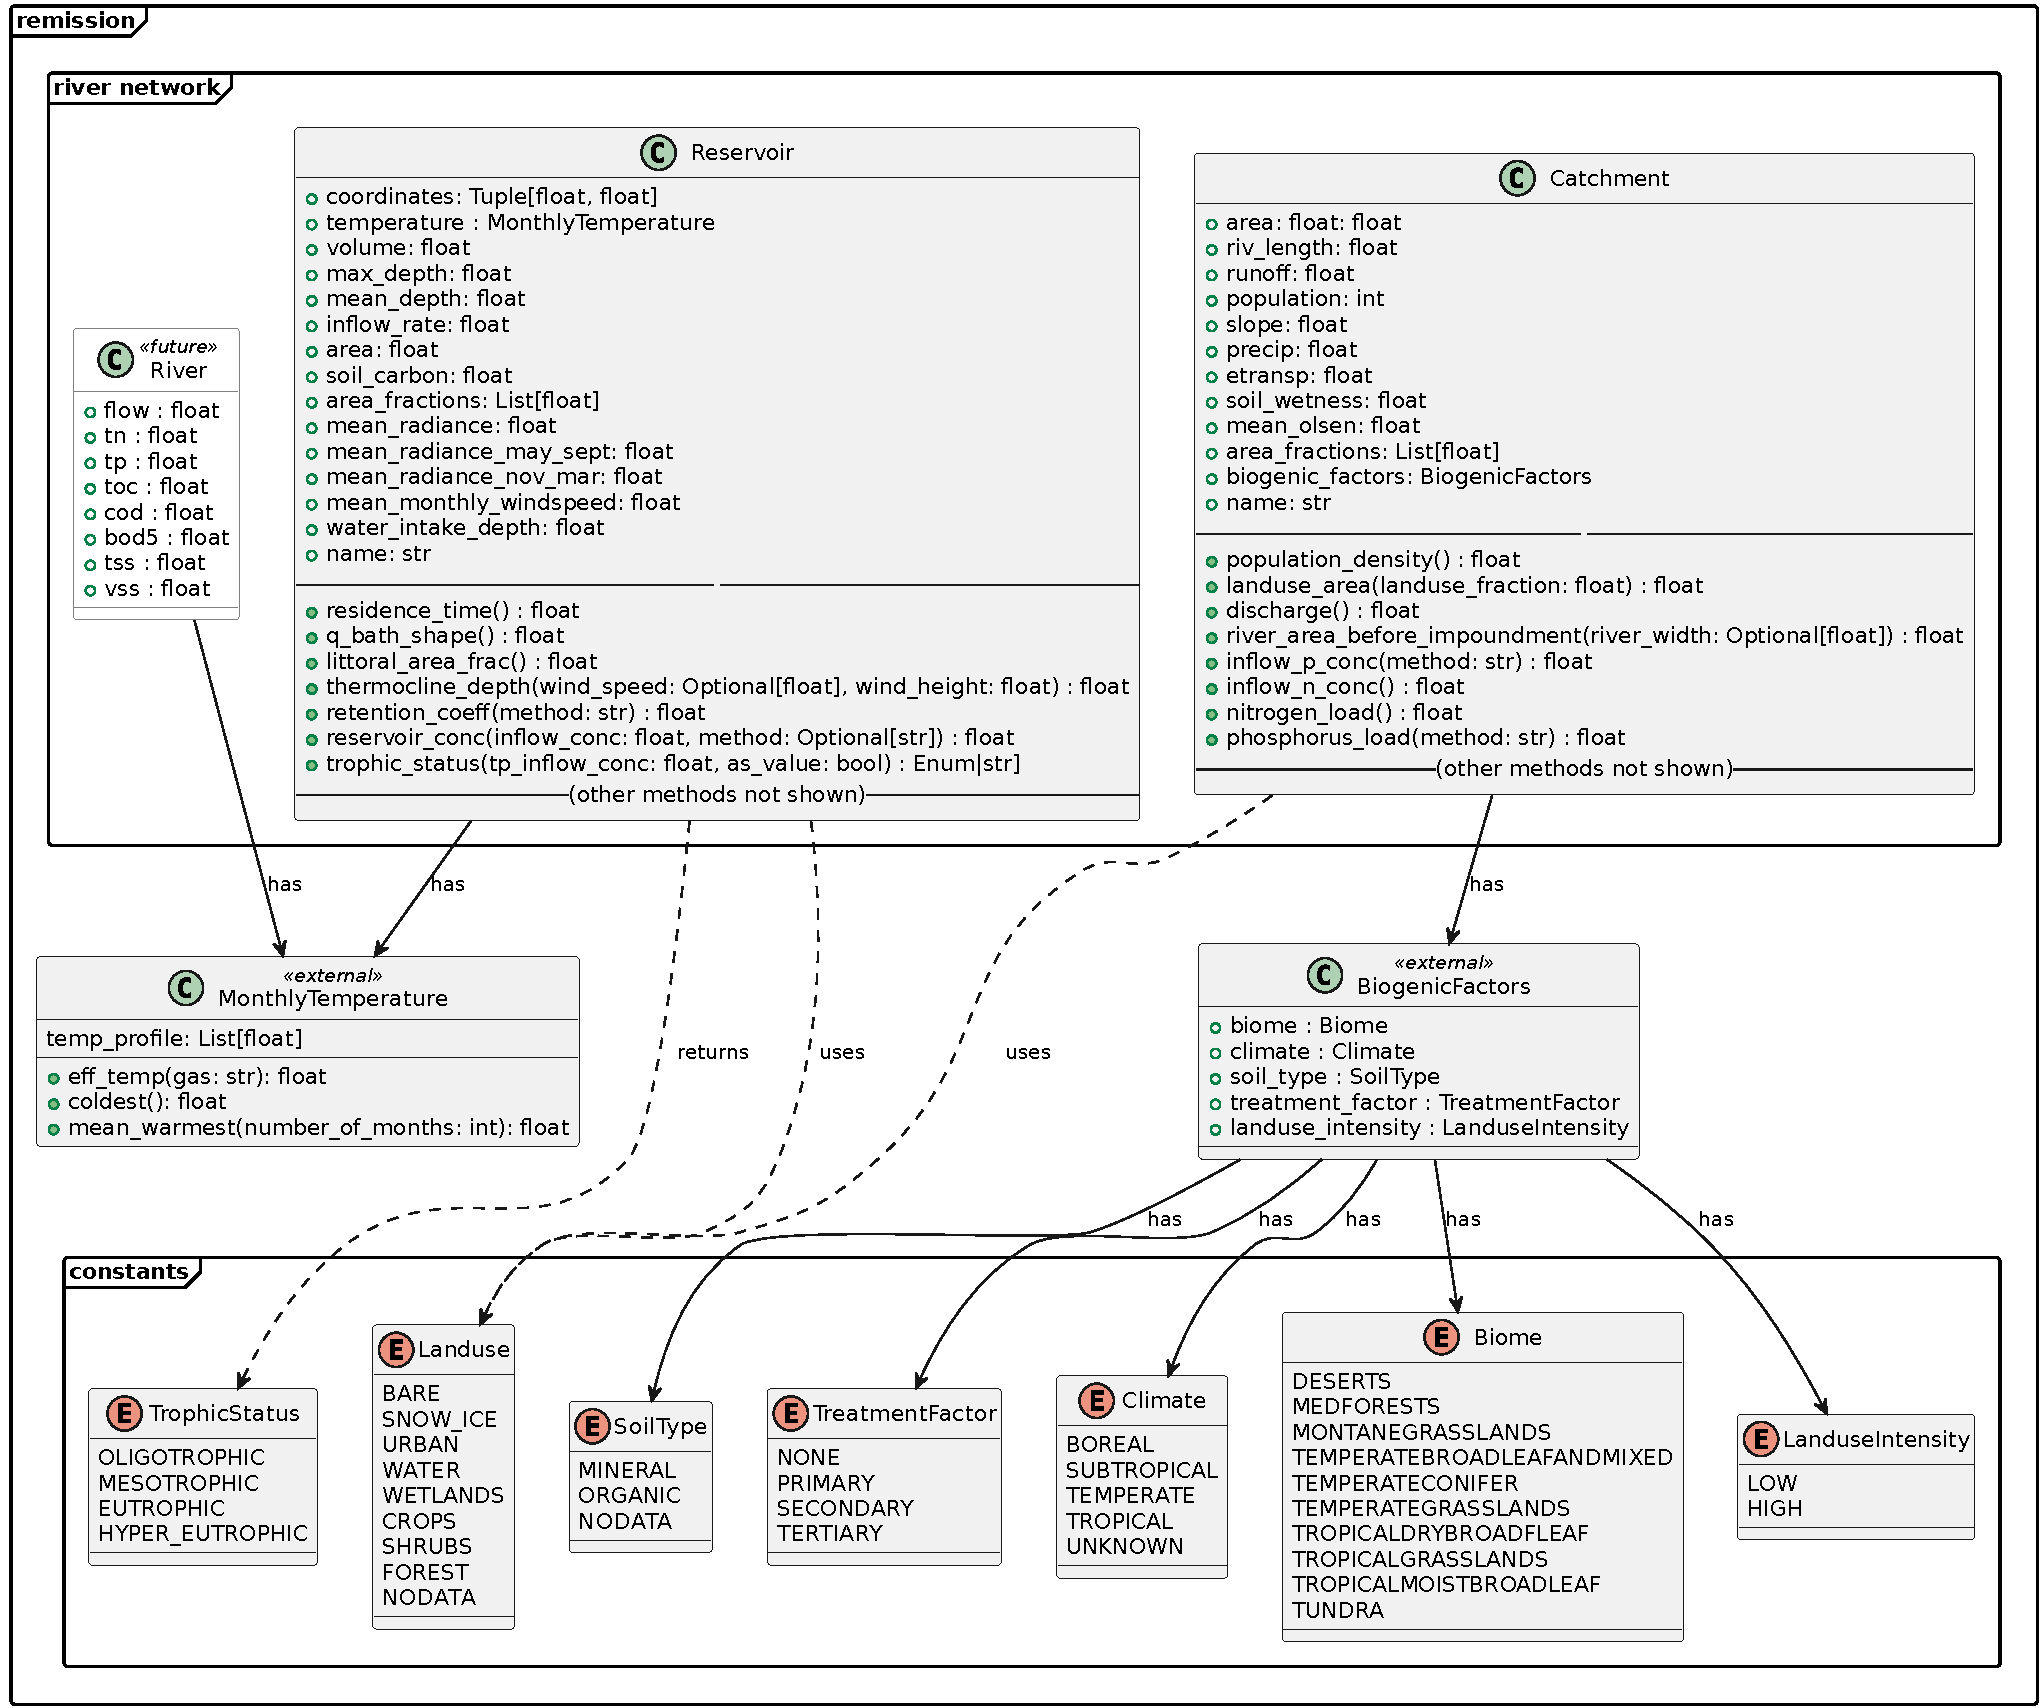
\includegraphics[width=0.99\textwidth]{figures/river_network_uml.pdf}
    \caption{A UML class diagram visualizing the \vrbbrk{Reservoir} and \vrbbrk{Catchment} classes and different container classes and categorical data representations using Enum classes.}
    \label{fig:river_network_emissions_uml}
\end{figure}

\begin{figure}[ht]
    \centering
    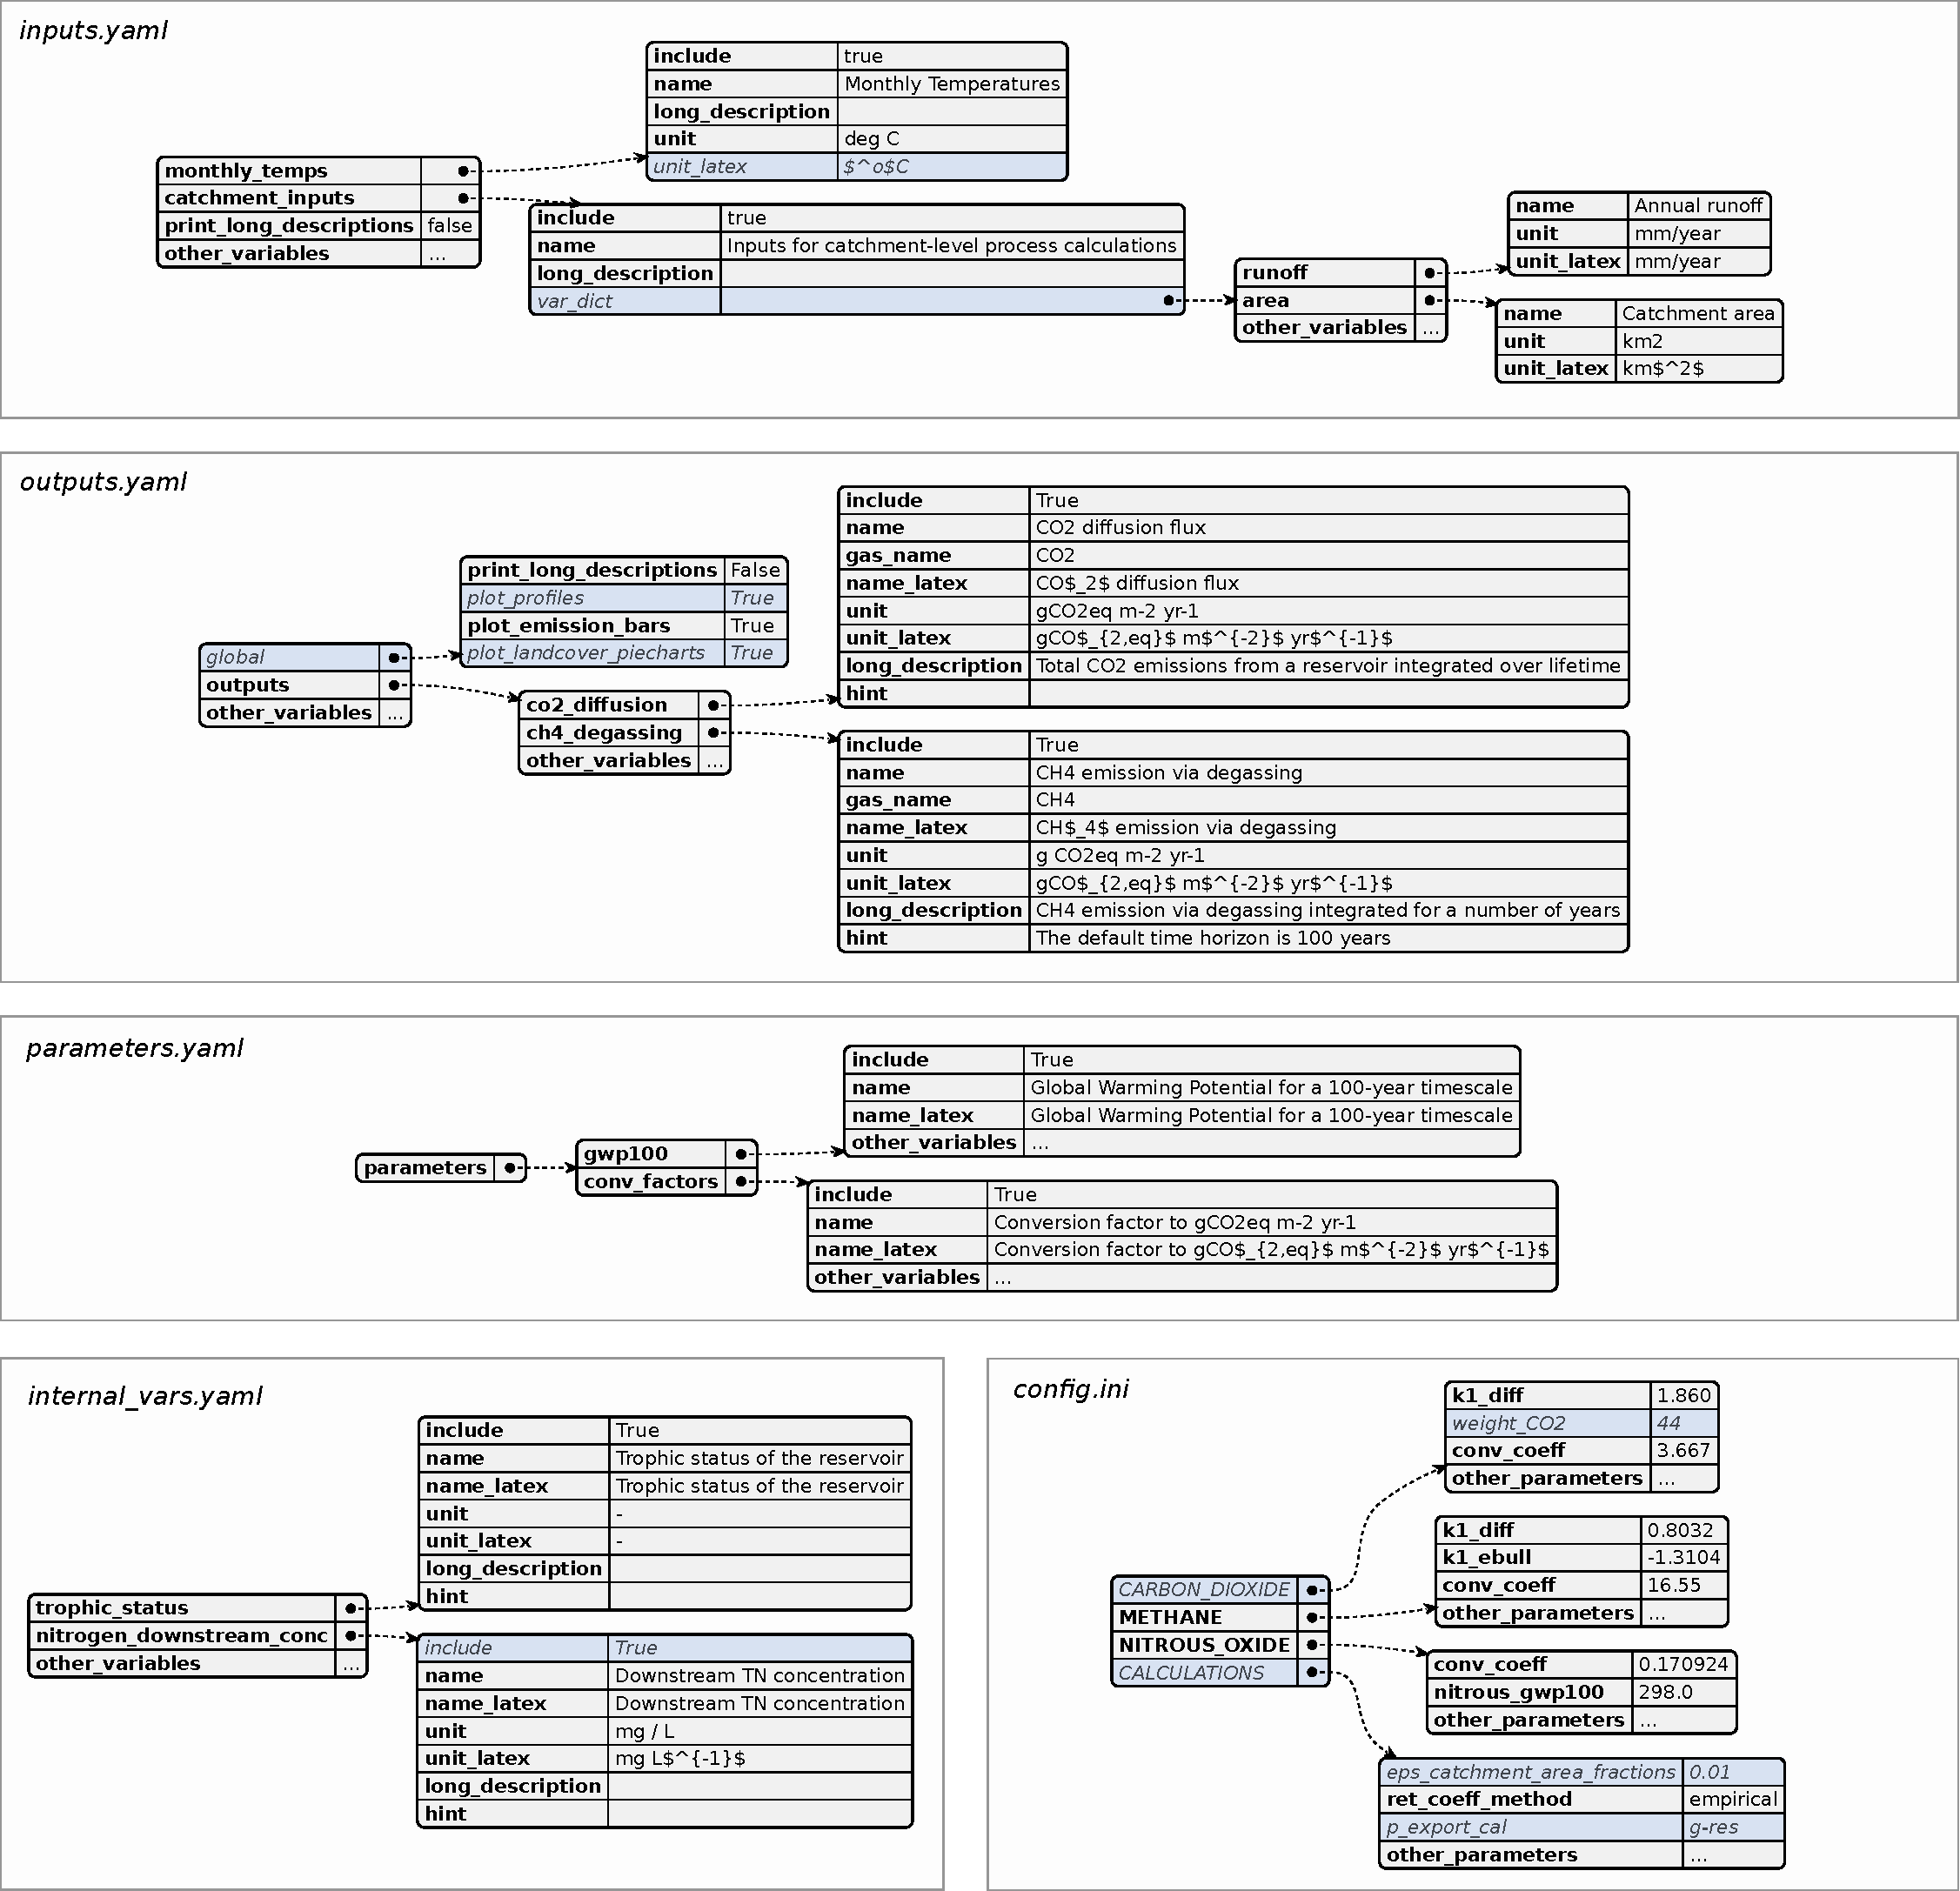
\includegraphics[width=0.99\textwidth]{figures/config_uml_portrait.pdf}
    \caption{Diagrams illustrating the structure of YAML configuration files used by the Presenter class (\vrbbrk{inputs.yaml}, \vrbbrk{outputs.yaml}, \vrbbrk{parameters.yaml}, \vrbbrk{internal\_vars.yaml}), along with the \vrbbrk{config.ini} file specifying emission model parameters and selection of alternative models.}
    \label{fig:config_uml}
\end{figure}

\begin{figure}[ht]
    \centering
    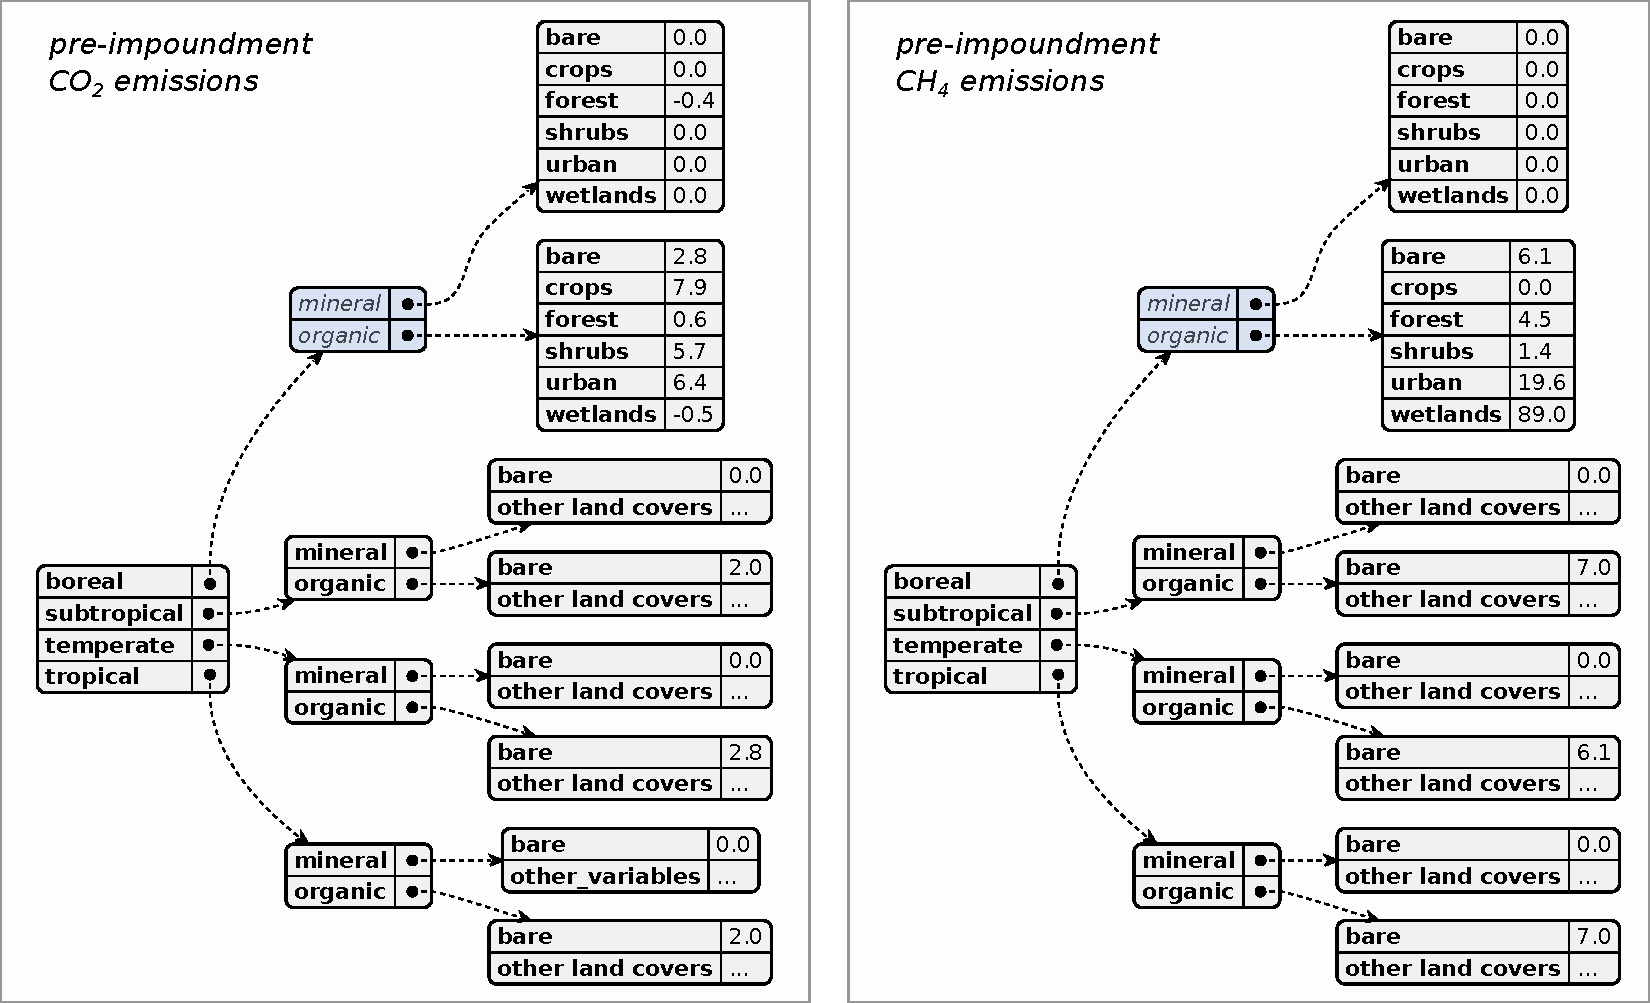
\includegraphics[width=0.80\textwidth]{figures/preimpoundment.pdf}
    \caption{Diagrams illustrating the structure of YAML configuration files and the underlying data relating areal pre-impoundment CO$_2$ and CH$_4$ emissions to climate, soil type, and land cover type.}
    \label{fig:preimpoundment}
\end{figure}

\begin{figure}[ht]
    \centering
    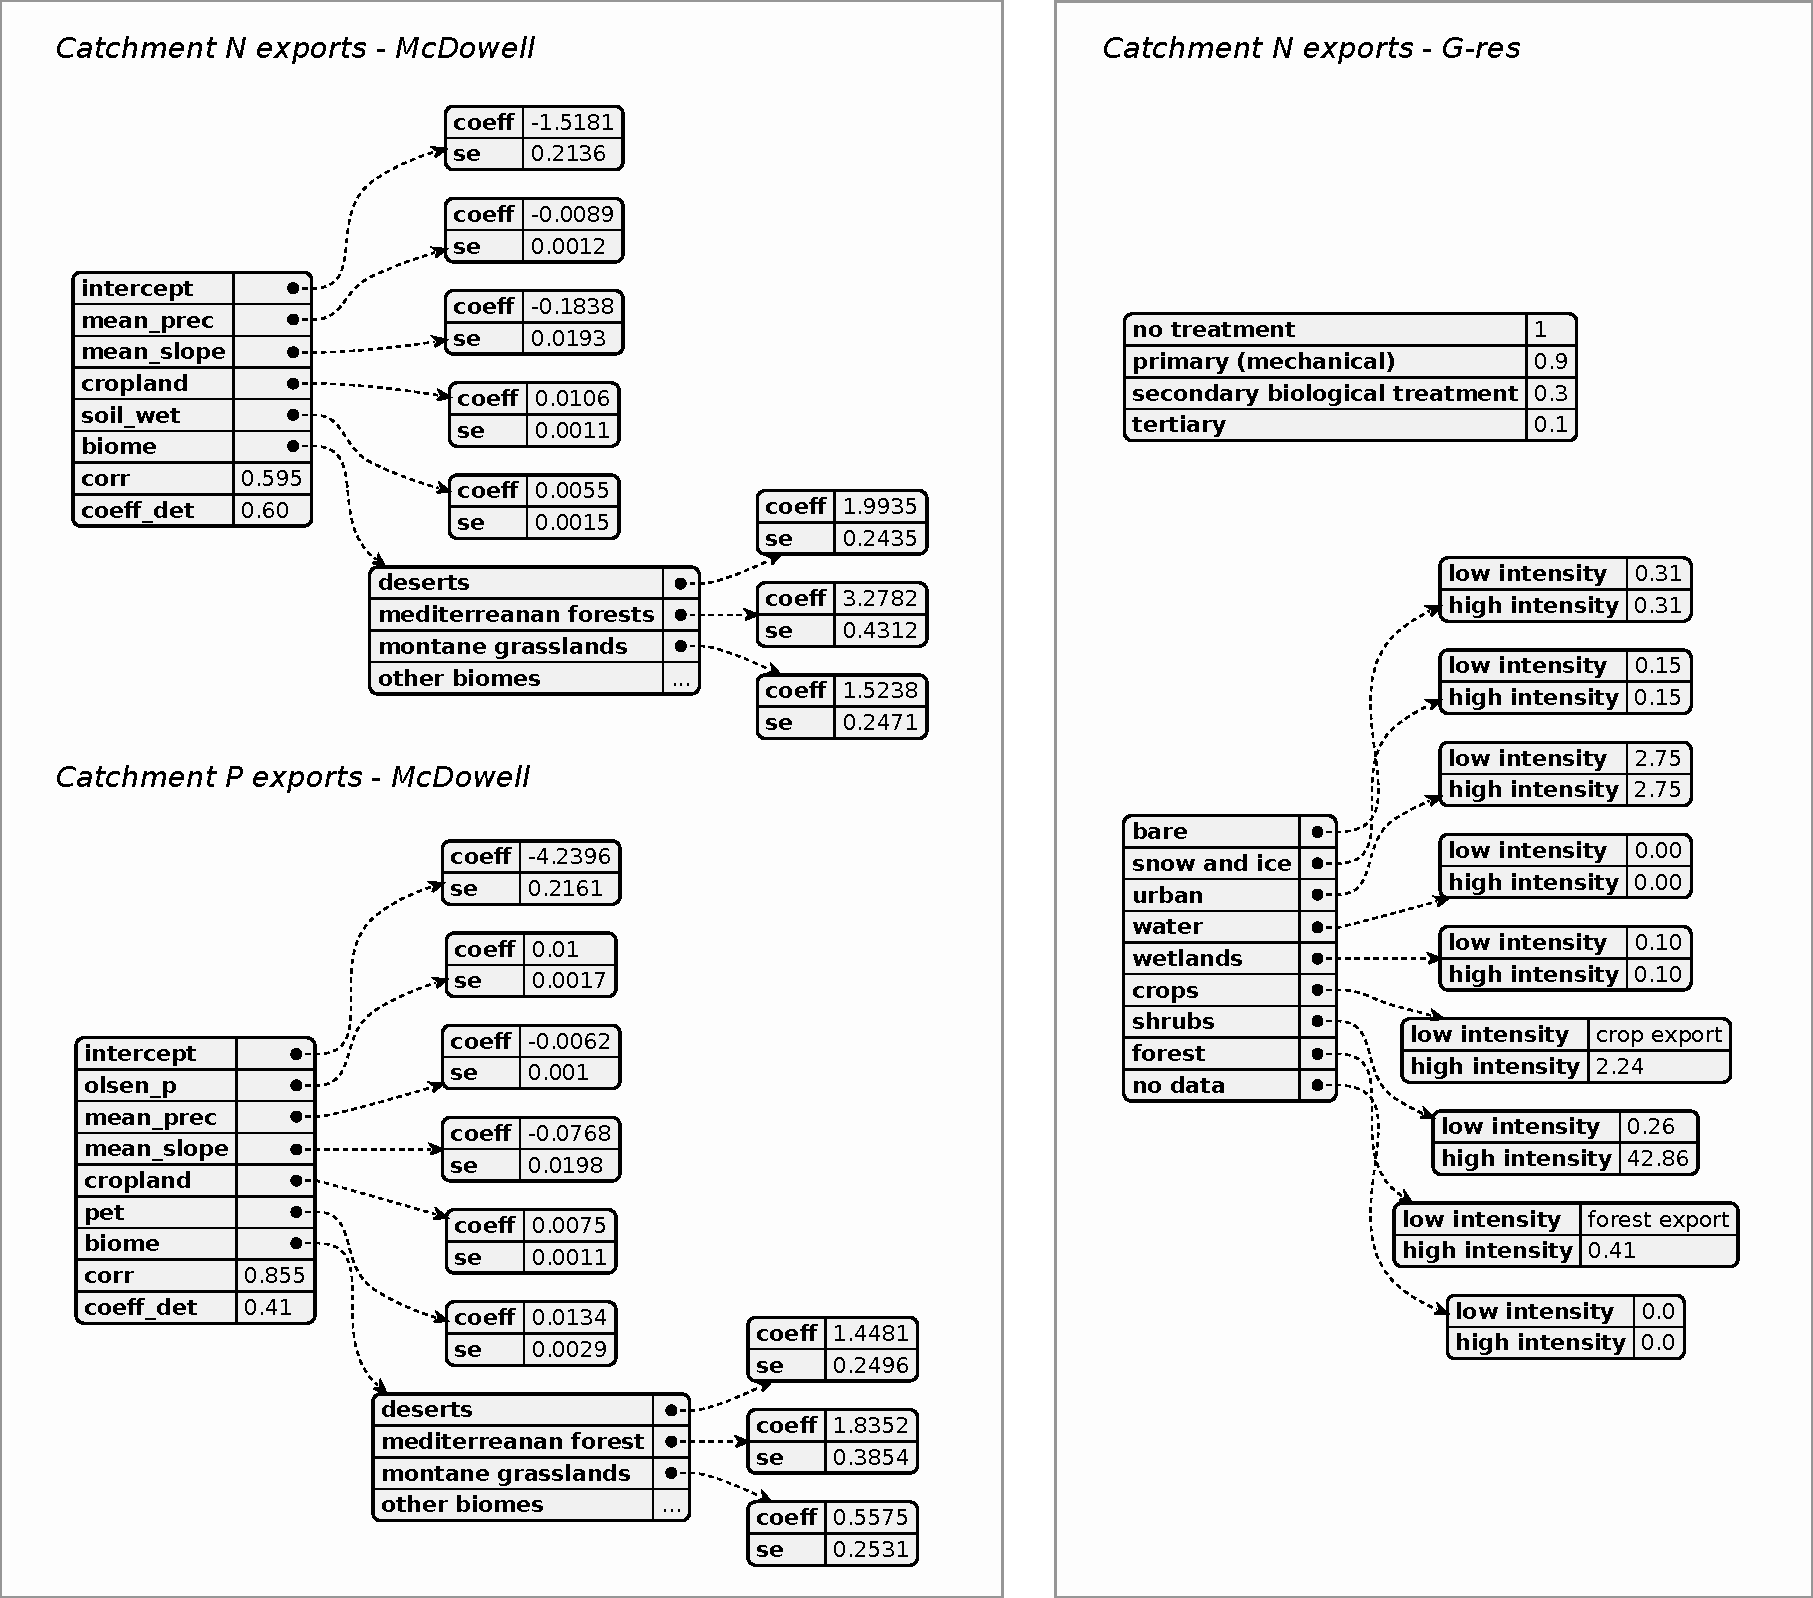
\includegraphics[width=0.85\textwidth]{figures/tp_tn_exports.pdf}
    \caption{Diagrams illustrating the structure of YAML configuration files parameterizing the nutrient export models of \citet{McDowell2020} (\ac{N} and \ac{P}) and G-res (\ac{N}).}
    \label{fig:tp_tn_exports}
\end{figure}

\begin{table}[ht]
	\small
    \caption{Input variables used by Re-Emission for estimating \ac{GHG} emissions from reservoirs}
    \label{app_table:input_variables}%
    \begin{tabular*}{\linewidth}{@{\extracolsep{\fill}}lc@{}}
    \toprule
    Input Name & Unit \\
    \midrule%
    \multicolumn{2}{c}{Inputs for catchment{-}level calculations}\\%
    %\midrule%
    Biome&{-} \\%
    Climate&{-} \\%
    Soil Type&{-} \\%
    Treatment Factor&{-}\\%
    Landuse Intensity&{-}\\%
    Monthly Temperatures&$^o$C\\%
    Annual runoff&mm/year\\%
    Catchment area&km$^2$\\%
    Length of inundated river&km\\%
    Population&capita\\%
    Area fractions\footnotemark[1]&--\\%
    Mean catchment slope&\%\\%
    Mean annual precipitation&mm/year\\%
    Mean annual evapotranspiration&mm/year\\%
    Soil wetness&mm over profile\\%
    Soil Olsen P content&kgP ha$^{-1}$\\%
    \midrule%
    \multicolumn{2}{c}{Inputs for reservoir{-}level calculations}\\%
    %\midrule%
    Reservoir volume&m$^3$\\%
    Reservoir area&km$^2$\\%
    Maximum reservoir depth&m\\%
    Mean reservoir depth&m\\%
    Inundated area fractions\footnotemark[1]&-\\%
    Soil carbon in inundated area&kgC m$^{-2}$\\%
    Mean monthly horizontal radiance&kWh m$^{-2}$ d$^{-1}$\\%
    Mean monthly horizontal radiance: May {-} Sept&kWh m$^{-2}$ d$^{-1}$\\%
    Mean monthly horizontal radiance: Nov {-} Mar&kWh m$^{-2}$ d$^{-1}$\\%
    Mean monthly wind speed&m s$^{-1}$\\%
    Water intake depth below surface&m\\
    \bottomrule
    \end{tabular*}
    \footnotetext[1]{Fractions of land cover in the delineated area.}
    \label{reemission_table}
\end{table}

%\FloatBarrier

\begin{acronym}
	\acro{ASEAN}{Association of Southeast Asian Nations}
	\acro{BRT}{Boosted Regression Tree}
	\acro{CO2}[CO$_2$]{carbon dioxide}
	\acro{CH4}[CH$_4$]{methane}
	\acro{CI}{continuous integration}
	%\acro{CI}{carbon intensity}
	\acro{CLI}{command line interface}
	\acro{DEM}{digital elevation model}
	\acro{DOC}{dissolved organic carbon}
	\acro{DOF}{degree of fragmentation}
	\acro{DOR}{degree of regulation}
	\acro{EF}{emission factor}
	\acro{EFDC}{Environmental Fluid Dynamics Code}
	\acro{EI}{emission intensity}
	\acro{EPA}{U.S. Environmental Protection Agency}
	\acro{ET}{evapotranspiration}
	\acro{FHReD}{High-Resolution Global Database of Dams}
	\acro{FSL}{full supply level}
	\acro{GDrive}{Google Drive}
	\acro{GGRP}{Greenhouse Gas Reporting Program}
	\acro{GEE}{Google Earth Engine}
	\acro{GHCR}{GitHub Container Registry}
    \acro{GHG}{greenhouse gas}    
	\acro{GIS}{geographical information system}
	\acro{G-res}{GHG Reservoir Tool}
	\acro{GOOD2}{Global geOreferenced Database of Dams}
	\acro{GW}{gigawatts}
	\acro{HP}{hydropower}
	\acro{ICOLD}{International Commission on Large Dams}
	\acro{IHA}{International Hydropower Association}
	\acro{KDE}{kernel density estimate}
	\acro{IPCC}{Intergovernmental Panel on Climate Change}
	\acro{KNN}{K-Nearest Neighbours Regressor}
	\acro{LCA}{life-cycle assessment}
	\acro{ML}{machine-learning}
	\acro{MW}{megawatts}
	\acro{MOEA}{multiobjective evolutionary algorithm}
	\acro{MOO}{multiobjective optimization}
	\acro{N}{Nitrogen}
	\acro{N2O}[N$_2$O]{nitrous oxide}
	\acro{P}{Phosphorus}
	\acro{PD}{partial-dependence}
	\acro{PPA}{power purchase agreement}
	\acro{PV}{Photovoltaic}
	\acro{RF}{Random Forest}
	\acro{ROI}{region of interest}
	\acro{RoR}{run-of-river}
	\acro{RMSE}{root-mean-square-error}
	\acro{SA}{sensitivity analysis}
	\acro{SDG}{sustainable development goal}
	\acro{SES}{social and ecological system}
	\acro{SVR}{Support Vector Regression}
	\acro{xAI}{explainable artificial-intelligence}
	\acro{TN}{Total Nitrogen}
	\acro{TP}{Total Phosphorus}
	\acro{UAS}{Unrelated Anthropogenic Sources}
    \acro{VRE}{variable renewable energy}
	\acro{WEFE}{Water-Energy-Food-Ecosystems}
	\acro{WRT}{water residence time}
\end{acronym}

\bibliographystyle{unsrtnat}
\bibliography{reemission}

\end{document}

\endinput
%%
%% End of file `elsarticle-template-num.tex'.
